\let\negmedspace\undefined
\let\negthickspace\undefined
\documentclass[journal,12pt,onecolumn]{IEEEtran}
\usepackage{cite}
\usepackage{amsmath,amssymb,amsfonts,amsthm}
\usepackage{algorithmic}
\usepackage{graphicx}
\usepackage{textcomp}
\usepackage{xcolor}
\usepackage{txfonts}
\usepackage{listings}
\usepackage{enumitem}
\usepackage{mathtools}
\usepackage{gensymb}
\usepackage{comment}
\usepackage[breaklinks=true]{hyperref}
\usepackage{tkz-euclide} 
\usepackage{listings}
\usepackage{gvv}                                        
%\def\inputGnumericTable{}                                 
\usepackage[utf8]{inputenc}

\usepackage{xparse}
\usepackage{color}                                            
\usepackage{array}                                            
\usepackage{longtable}                                       
\usepackage{calc}                                             
\usepackage{multirow}
\usepackage{multicol}
\usepackage{hhline}                                           
\usepackage{ifthen}                                           
\usepackage{lscape}
\usepackage{tabularx}
\usepackage{array}
\usepackage{float}
\newtheorem{theorem}{Theorem}[section]
\newtheorem{problem}{Problem}
\newtheorem{proposition}{Proposition}[section]
\newtheorem{lemma}{Lemma}[section]
\newtheorem{corollary}[theorem]{Corollary}
\newtheorem{example}{Example}[section]
\newtheorem{definition}[problem]{Definition}
\newcommand{\BEQA}{\begin{eqnarray}}
\newcommand{\EEQA}{\end{eqnarray}}
\usepackage{float}
%\newcommand{\define}{\stackrel{\triangle}{=}}
\theoremstyle{remark}
\usepackage{ circuitikz }
\begin{document}

\title{2013 XE}
\author{EE25BTECH11021 - Dhanush sagar}
\maketitle
\renewcommand{\thefigure}{\theenumi}
\renewcommand{\thetable}{\theenumi}
\title{2017 Xe}
\author{Dhanush Sagar}
\date{August 2025}
\begin{enumerate}

 
    % Q1
    \item If
    \begin{align}
        \int_{0}^{\frac{\pi}{\alpha}} \frac{\sin y}{y}\, dy = \frac{1}{2}
    \end{align}
    for some $\alpha \geq 1$, then the value of $\alpha$ is \_\_\_\_\_.
    \hfill [GATE 2017 XE]

    % Q2
    \item Three fair dice are rolled simultaneously. The probability of getting a sum of 5 is
    \begin{multicols}{4}
    \begin{enumerate}
        \item $\tfrac{1}{108}$
        \item $\tfrac{1}{72}$
        \item $\tfrac{1}{54}$
        \item $\tfrac{1}{36}$
    \end{enumerate}
    \end{multicols}
    \hfill [GATE 2017 XE]

    % Q3
    \item Suppose $\alpha, \beta, \gamma, \delta$ are constants such that
    \begin{align}
        p(x) &= \delta + \gamma(x+1) + \beta(x+1)(x-1) + \alpha(x+1)(x-1)(x-2)
    \end{align}
    is the interpolating polynomial for the data $(-1,-3), (0,1), (1,-1), (2,-3)$.  
    Then the value of $\beta - \alpha$ is \_\_\_\_\_.
    \hfill [GATE 2017 XE]

    % Q4
    \item Consider the ordinary differential equation
    \begin{align}
        y^{\prime\prime\prime} + \alpha y^{\prime} + \beta y = 0
    \end{align}
    where $\alpha$ and $\beta$ are constants. If $y(x) = x e^x$ is a solution of the above equation,  
    then the value of $\beta - \alpha$ is \_\_\_\_\_.
    \hfill [GATE 2017 XE]

    % Q5
    \item Consider the system of linear equations
    \begin{align}
        2x_2 + x_3 &= 0, \\
        -2x_1 - x_3 &= 0, \\
        -x_1 + x_2 &= 1.
    \end{align}
    The above system has
    \begin{multicols}{2}
    \begin{enumerate}
        \item a unique solution
        \item infinite number of solutions
        \item no solution
        \item only two distinct solutions
    \end{enumerate}
    \end{multicols}
    \hfill [GATE 2017 XE]

    % Q6
    \item Let $C$ be a simple smooth closed curve enclosing the region $R$ in the $xy$-plane.  
    Let $C$ be oriented counterclockwise. If the value of the integral
    \begin{align}
        \iint_{R} \left( y + e^{x^2}\right) dx + \left(3x + \cos y\right) dy
    \end{align}
    is $16$, then the area of $R$ is \_\_\_\_\_.
    \hfill [GATE 2017 XE]
\item Consider the ordinary differential equation
    \begin{align}
        x^2 y^{\prime\prime} + x y^{\prime} - y = x, \quad x > 0.
    \end{align}
    In terms of arbitrary constants $c_1, c_2$, the general solution of the above equation is
    \begin{multicols}{2}
    \begin{enumerate}
        \item $c_1 x + c_2 x^{-1} + \tfrac{1}{3}x^2$
        \item $c_1 x + c_2 x^{-1} + \tfrac{1}{2}x$
        \item $c_1 x + c_2 x^{-1} + \tfrac{1}{4}x^2$
        \item $c_1 x + c_2 x^{-1} + \tfrac{1}{2}x^2$
    \end{enumerate}
    \end{multicols}
    \hfill [GATE 2017 XE]

    % Q8
    \item Let $f:\mathbb{R} \to \mathbb{R}$ and $g:\mathbb{R} \to \mathbb{R}$ be defined by
    \begin{align}
        f(x) &= \begin{cases}
        (x \sin \tfrac{1}{x}), & x \neq 0, \\
        0, & x = 0,
        \end{cases} \\
        g(x) &= \begin{cases}
        \cos \tfrac{1}{x}, & x \neq 0, \\
        0, & x = 0,
        \end{cases}
    \end{align}
    where $\mathbb{R}$ denotes the set of real numbers. Then at $x=0$
    \begin{multicols}{2}
    \begin{enumerate}
        \item $f$ is differentiable but $g$ is not differentiable
        \item Both $f$ and $g$ are differentiable
        \item Neither $f$ nor $g$ is differentiable
        \item Only $g$ is differentiable
    \end{enumerate}
    \end{multicols}
    \hfill [GATE 2017 XE]

    % Q9
    \item If $u(x,t) = g(t) \sin x$ is the solution of the wave equation
    \begin{align}
        \frac{\partial^2 u}{\partial t^2} &= \frac{\partial^2 u}{\partial x^2}, \quad 0 < x < \pi,
    \end{align}
    with initial conditions
    \begin{align}
        u(x,0) &= 2 \sin x, \quad u_t(x,0) = 0, \quad 0 \leq x \leq \pi,
    \end{align}
    and the boundary conditions
    \begin{align}
        u(0,t) = 0, \quad u(\pi,t) = 0, \quad t \geq 0,
    \end{align}
    then the value of $g(\tfrac{\pi}{6})$ is \_\_\_\_\_.
    \hfill [GATE 2017 XE]

    % Q10
    \item Let
    \begin{align}
        I = \int_{-1}^{1} \frac{e^t}{1+e^t}\,dt + \int_{-1}^{1} \frac{1}{1+e^t}\,dt.
    \end{align}
    If $x$ is a real variable and $I = \tfrac{1}{x} \int_{-1}^{1} e^t\, dt$,  
    then the value of $x$ is \_\_\_\_\_.
    \hfill [GATE 2017 XE]

    % Q11
    \item Let $a_n = 2^n + \sin n$, and $b_n = 2^n + n \sin^2 n$, for $n = 1,2,\ldots$.  
    Then
    \begin{multicols}{2}
    \begin{enumerate}
        \item Both $\sum a_n$ and $\sum b_n$ diverge
        \item $\sum a_n$ converges but $\sum b_n$ does NOT converge
        \item $\sum a_n$ does NOT converge but $\sum b_n$ converges
        \item Both $\sum a_n$ and $\sum b_n$ converge
    \end{enumerate}
    \end{multicols}
    \hfill [GATE 2017 XE]

\item The event would have been successful if you \underline{\hspace{2cm}} able to come.  
\hfill [GATE 2017 XE]

\begin{multicols}{2}
\begin{enumerate}
    \item are
    \item had been
    \item have been
    \item would have been
\end{enumerate}
\end{multicols}

% Q167
\item There was no doubt that their work was \underline{thorough}.  
Which of the words below is closest in meaning to the underlined word above?  
\hfill [GATE 2017 XE]

\begin{multicols}{2}
\begin{enumerate}
    \item pretty
    \item complete
    \item sloppy
    \item haphazard
\end{enumerate}
\end{multicols}

% Q168
\item Four cards lie on a table. Each card has a number printed on one side and a colour on the other.  
The faces visible on the cards are 2, 3, red, and blue.  

Proposition: If a card has an even value on one side, then its opposite face is red.  

The cards which MUST be turned over to verify the above proposition are  
\hfill [GATE 2017 XE]

\begin{multicols}{2}
\begin{enumerate}
    \item 2, red
    \item 2, 3, red
    \item 2, blue
    \item 2, red, blue
\end{enumerate}
\end{multicols}

% Q169
\item What is the value of $x$ when
\begin{align}
81 \times \left(\frac{25}{81}\right)^{x+2} + \left(\frac{25}{81}\right)^{2x+4} = 144?
\end{align}
\hfill [GATE 2017 XE]

\begin{multicols}{2}
\begin{enumerate}
    \item 1
    \item -1
    \item -2
    \item Cannot be determined
\end{enumerate}
\end{multicols}

% Q170
\item Two dice are thrown simultaneously. The probability that the product of the numbers appearing on the top faces of the dice is a perfect square is  
\hfill [GATE 2017 XE]

\begin{multicols}{2}
\begin{enumerate}
    \item $\tfrac{1}{9}$
    \item $\tfrac{2}{9}$
    \item $\tfrac{1}{3}$
    \item $\tfrac{4}{9}$
\end{enumerate}
\end{multicols}

% Q171
\item Bhaichung was observing the pattern of people entering and leaving a car service centre.  
There was a single window where customers were being served. He saw that people invariably came out of the centre in the order that they went in.  
However, the time they spent inside seemed to vary a lot: some people came out in a matter of minutes while for others it took much longer.  

From this, what can one conclude?  
\hfill [GATE 2017 XE]

\begin{enumerate}
    \item The centre operates on a first-come-first-served basis, but with variable service times.  
    \item Customers were served in an arbitrary order, since they took varying amounts of time for service completion in the centre.  
    \item Since some people came out within a few minutes of entering the centre, the system is likely to operate on a last-come-first-served basis.  
    \item Entering the centre early ensured that one would have shorter service times and most people attempted to do this.  
\end{enumerate}

\item A map shows the elevations of Darjeeling, Gangtok, Kalimpong, Pelling, and Siliguri.  
Kalimpong is at a lower elevation than Gangtok. Pelling is at a lower elevation than Gangtok.  
Pelling is at a higher elevation than Siliguri. Darjeeling is at a higher elevation than Gangtok.  

Which of the following statements can be inferred from the paragraph above?  
\hfill [GATE 2017 XE]

i. Pelling is at a higher elevation than Kalimpong  \\
ii. Kalimpong is at a lower elevation than Darjeeling  \\
iii. Kalimpong is at a higher elevation than Siliguri  \\
iv. Siliguri is at a lower elevation than Gangtok  \\

\begin{multicols}{2}
\begin{enumerate}
    \item Only ii
    \item Only ii and iii
    \item Only ii and iv
    \item Only iii and iv
\end{enumerate}
\end{multicols}

% Q173
\item P, Q, R, S, T and U are seated around a circular table.  
R is seated two places to the right of Q. P is seated three places to the left of R. S is seated opposite U.  
If P and U now switch seats, which of the following must necessarily be true?  
\hfill [GATE 2017 XE]

\begin{multicols}{2}
\begin{enumerate}
    \item P is immediately to the right of R
    \item T is immediately to the left of P
    \item T is immediately to the left of P or P is immediately to the right of Q
    \item U is immediately to the right of R or P is immediately to the left of T
\end{enumerate}
\end{multicols}

% Q174
\item Badhan covers a distance of 19 km in 2 hours by cycling one fourth of the time and walking the rest.  
The next day he cycles (at the same speed as before) for half the time and walks the rest (at the same speed as before) and covers 26 km in 2 hours.  
The speed in km/h at which Badhan walks is \underline{\hspace{2cm}}.  
\hfill [GATE 2017 XE]

\begin{multicols}{2}
\begin{enumerate}
    \item 1
    \item 4
    \item 5
    \item 6
\end{enumerate}
\end{multicols}

% Q175
\item The points in the graph below represent the halts of a lift for durations of 1 minute, over a period of 1 hour.  

\begin{figure}[H]
    \centering
    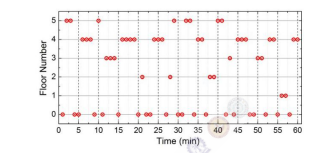
\includegraphics[width=0.5\linewidth]{figs/fig1.png}
    \caption{}
    \label{fig:fig1}
\end{figure}

Which of the following statements are correct?  
\hfill [GATE 2017 XE]

i. The elevator never moves directly from any non-ground floor to another non-ground floor.\\  
ii. The lift halts on the 2nd floor for the longest duration over the one hour period.  

\begin{multicols}{2}
\begin{enumerate}
    \item Only i
    \item Only ii
    \item Both i and ii
    \item Neither i nor ii
\end{enumerate}
\end{multicols}
\item In a given flow field, the velocity vector in Cartesian coordinate system is given as:
\begin{align}
\vec{V} = \left( x^2 + y^2 + z^2 \right)\hat{i} + \left( y^2 + xy + x^2 \right)\hat{j} + \left( yz + z^2 \right)\hat{k}
\end{align}
What is the volume dilatation rate of the fluid at a point where $x = 1, y = 2, z = 3$?  
\hfill [GATE 2017 XE]

\begin{multicols}{2}
\begin{enumerate}
    \item 6
    \item 10
    \item 16
    \item 20
\end{enumerate}
\end{multicols}

% Q13
\item A steady, incompressible, two-dimensional velocity field in Cartesian coordinate system is represented by the following expression:
\begin{align}
\vec{V} = (0.7 + 0.4x)\hat{i} + (0.2 - 0.4y)\hat{j}
\end{align}
The coordinates of one possible stagnation point of the velocity field are  
\hfill [GATE 2017 XE]

\begin{multicols}{2}
\begin{enumerate}
    \item (0.7, 0.5)
    \item (-0.5, 0.5)
    \item (0.7, -0.5)
    \item (-0.5, -0.5)
\end{enumerate}
\end{multicols}

% Q14
\item During an experiment, the position of a fluid particle is monitored by an instrument over a time period of 10 s. The trace of the particle given by the following figure represents a

\begin{figure}[H]
    \centering
    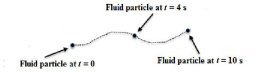
\includegraphics[width=0.5\linewidth]{figs/fig2.png}
    \caption{}
    \label{fig:fig2}
\end{figure}

\hfill [GATE 2017 XE]

\begin{multicols}{2}
\begin{enumerate}
    \item Streakline
    \item Pathline
    \item Streamline
    \item Timeline
\end{enumerate}
\end{multicols}

% Q15
\item In a Cartesian two-dimensional coordinate system, $x$ and $y$ represent the velocities in $x$ and $y$ directions respectively.  
For a certain flow, the velocity field is represented by the following expression:
\begin{align}
\vec{V} = (ax + by)\hat{i} + (cx + dy)\hat{j}
\end{align}
where the coefficients $a,b,c,d$ are constants. For an incompressible flow, which one of the following conditions is TRUE?  
\hfill [GATE 2017 XE]

\begin{multicols}{2}
\begin{enumerate}
    \item $a + d = 0$
    \item $b + c = 0$
    \item $a + c = 0$
    \item $b + d = 0$
\end{enumerate}
\end{multicols}

% Q16
\item Which one of the following figures represents potential flow past a circular cylinder with clockwise circulation of the cylinder?  
\hfill [GATE 2017 XE]

\begin{figure}[H]
    \centering
    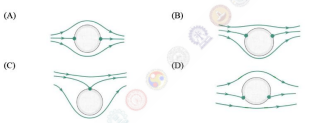
\includegraphics[width=0.5\linewidth]{figs/fig3.png}
    \caption{}
    \label{fig:fig3}
\end{figure}

% Q17
\item The vorticity function $\omega$ of a velocity field at any location is $(x,y)$ is given as,  
\begin{align}
\omega = y^2 + 2x^2 y
\end{align}
What is the rate of rotation of a fluid element located between $x=2,y=2$ ?  
\hfill [GATE 2017 XE]

\begin{multicols}{2}
\begin{enumerate}
    \item 14
    \item 10
    \item 8
    \item 12
\end{enumerate}
\end{multicols}

% Q18
\item The trace of velocity potential within the laminar viscous sublayer in a turbulent pipe flow is  
\hfill [GATE 2017 XE]

\begin{multicols}{2}
\begin{enumerate}
    \item Linear
    \item Log-parabolic
    \item Logarithmic
    \item Exponential
\end{enumerate}
\end{multicols}

\item In a 5 m deep vertical cylindrical tank, water is filled up to a level of 3 m from the bottom and the remaining space is filled with oil of specific gravity 0.88.  
Assume density of water as $1000 \,\text{kg/m}^3$ and acceleration due to gravity to be $10 \,\text{m/s}^2$.  

The gauge pressure (in kN/m$^2$, rounded off to the first decimal place) at a depth of 2.5 m from the top of the tank will be \underline{\hspace{2cm}}.  
\hfill [GATE 2017 XE]

% Q20
\item In a two-dimensional potential flow, a point source is located at the origin $(x = 0, y = 0)$ as shown in the figure.  
The strength of the point source is $2 \,\text{cm}^2/\text{s}$.  
A uniform flow with velocity $1 \,\text{cm/s}$ is approaching towards the point source at an angle of $30^\degree$ from the horizontal axis.  

What is the distance (cm) of the stagnation point in the flow field from the point source?  
\hfill [GATE 2017 XE]

\begin{figure}[H]
    \centering
    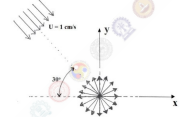
\includegraphics[width=0.5\linewidth]{figs/fig4.png}
    \caption{}
    \label{fig:fig4}
\end{figure}

\begin{multicols}{2}
\begin{enumerate}
    \item $\tfrac{1}{\pi}$
    \item $\tfrac{2}{\pi}$
    \item $\tfrac{1}{2\pi}$
    \item $\tfrac{\sqrt{3}}{2\pi}$
\end{enumerate}
\end{multicols}
\item Two infinite parallel horizontal plates are separated by a small gap ($h = 20 \,\text{mm}$) as shown in figure.  
The lower plate is fixed and the upper plate moves with a velocity of $40 \,\text{m/s}$, while the gap between the plates is filled with a Newtonian fluid of viscosity $\mu = 0.1 \,\text{Pa.s}$.  
Assume linear velocity distribution and no pressure gradient in the flow direction.  

The shear stress (N/m$^2$) on the upper plate is \underline{\hspace{2cm}}.  
\hfill [GATE 2017 XE]

\begin{figure}[H]
    \centering
    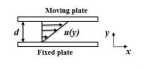
\includegraphics[width=0.5\linewidth]{figs/fig5.png}
    \caption{}
    \label{fig:fig5}
\end{figure}


\item A spherical balloon of diameter 15 m is supposed to lift a load of 3000 N. 
The lifting of load is achieved by heating the air inside the balloon. 
Assume, air to be an ideal gas and atmospheric pressure either outside or inside the balloon. 
The value of acceleration due to gravity is 9.81 m/s$^2$ and the values of temperature 
and density of atmospheric air are 15$^\degree$C and 1.2 kg/m$^3$, respectively. 
In order to lift the specified load, the air inside the balloon should be heated to a temperature (°C) of \underline{\hspace{2cm}}. 

\hfill [GATE 2017 XE]




\item The velocity field in Cartesian coordinate system for a two-dimensional steady flow is given as:
\begin{align}
    \vec{V} = \left( \frac{V_0}{L} \right) (x \hat{i} - y \hat{j})
\end{align}
where, $V_0$ and $L$ are constants. Which one of the following expressions represents the acceleration field ($\vec{a}$) for this flow?

\hfill [GATE 2017 XE]

\begin{enumerate}
\begin{multicols}{2}
    \item $\vec{a} = 0$
    \item $\vec{a} = \left( \frac{V_0}{L} \right) (x \hat{i} + y \hat{j})$
    \item $\vec{a} = \left( \frac{V_0^2}{L^2} \right) (x \hat{i} - y \hat{j})$
    \item $\vec{a} = \left( \frac{V_0^2}{L^2} \right) (x \hat{i} + y \hat{j})$
\end{multicols}
\end{enumerate}
\item A cylindrical tank of 0.8 m diameter is completely filled with water and its top surface is open to atmosphere as shown in the figure.  
Water is being discharged to the atmosphere from a circular hole of 15 mm diameter located at the bottom of the tank.  
The value of acceleration due to gravity is $9.81 \,\text{m/s}^2$.  

How much time (in seconds) would be required for water level to drop from a height of 1 m to 0.5 m?  
\hfill [GATE 2017 XE]

\begin{figure}[H]
    \centering
    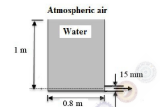
\includegraphics[width=0.5\linewidth]{figs/fig6.png}
    \caption{}
    \label{fig:fig6}
\end{figure}

\begin{multicols}{2}
\begin{enumerate}
    \item 188
    \item 266
    \item 376
    \item 642
\end{enumerate}
\end{multicols}

% Q25
\item Consider steady laminar flow of an incompressible Newtonian fluid between two infinite parallel plates, separated by a distance of 1 m, as shown in the figure.  
The bottom plate is stationary but the top one is moving in positive $x$-direction with a velocity of 3 m/s.  
The fluid pressure gradient in the flow direction is:  
\begin{align}
\frac{\partial P}{\partial x} = -18 \,\text{N/m}^3
\end{align}

If the viscosity of the fluid is $1 \,\text{kg/m.s}$ then the distance of the point of maximum velocity (in meters, rounded off to the second decimal place) from the bottom plate would be \underline{\hspace{2cm}}.  
\hfill [GATE 2017 XE]

\begin{figure}[H]
    \centering
    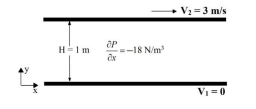
\includegraphics[width=0.5\linewidth]{figs/fig7.png}
    \caption{}
    \label{fig:fig7}
\end{figure}
% Q26
\item An inviscid incompressible fluid of density $1000 \,\text{kg/m}^3$ is flowing in a horizontal pipe of tapered cross-section with a flow rate of $4000 \,\text{cm}^3/\text{s}$.  
The area of cross-section at two different locations ‘A’ and ‘B’ are $10 \,\text{cm}^2$ and $20 \,\text{cm}^2$, respectively.  
The velocity of the fluid at the location ‘A’ is 4 m/s and pressure is $5 \,\text{N/cm}^2$.  

The pressure (N/m$^2$) at location ‘B’ would be \underline{\hspace{2cm}}.  
\hfill [GATE 2017 XE]

% Q27
\item A viscous, incompressible and Newtonian fluid flowing through the main branch of a circular pipe bifurcates into two daughter branches whose radii are $a$ cm and $2a$ cm, respectively.  
The flow in both the daughter branches are laminar and fully developed.  

If the pressure gradients in both the daughter branches are same, then the fraction of total volumetric flow rates (rounded off to the second decimal place) through the smaller branch to the larger branch is \underline{\hspace{2cm}}.  
\hfill [GATE 2017 XE]

\begin{figure}[H]
    \centering
    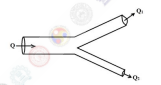
\includegraphics[width=0.5\linewidth]{figs/fig8.png}
    \caption{}
    \label{fig:fig8}
\end{figure}

\item The volumetric flow rate ($Q$) of a triangular notch is a function of the upstream liquid surface elevation ($H$) measured from the bottom of the notch, acceleration due to gravity ($g$), notch angle ($\theta$) and the approach velocity ($V$).  

Which one of the following is the correct expression for $Q$?  
\hfill [GATE 2017 XE]

\begin{multicols}{2}
\begin{enumerate}
    \item $Q = H^{\tfrac{5}{2}}\sqrt{gH}\sqrt{\tan \tfrac{\theta}{2}}$
    \item $Q = H^{\tfrac{3}{2}}\sqrt{\tfrac{gH}{V}} \sqrt{\tan \tfrac{\theta}{2}}$
    \item $Q = H^{\tfrac{3}{2}}\sqrt{\tfrac{V}{gH}} \sqrt{\tan \tfrac{\theta}{2}}$
    \item $Q = H^{\tfrac{5}{2}}\sqrt{V} \sqrt{\tan \tfrac{\theta}{2}}$
\end{enumerate}
\end{multicols}

% Q29
\item Model tests are to be carried out to study the flow through a large prototype valve of 0.6 m diameter at a flow rate of 10 m$^3$/s.  
The same working fluid is used for both the model and the prototype.  
A complete geometric similarity is maintained between the model and the prototype.  
If the valve diameter of the model is 80 mm, its required flow rate (in m$^3$/s, rounded off to the first decimal place) would be \underline{\hspace{2cm}}.  
\hfill [GATE 2017 XE]

% Q30
\item Water is flowing at a rate of 0.6 m$^3$/s in a horizontal pipeline of inside diameter 0.3 m.  
The density and kinematic viscosity of water are $1000 \,\text{kg/m}^3$ and $10^{-6} \,\text{m}^2/\text{s}$, respectively.  
Assume Darcy-Weisbach friction factor for the flow to be 0.02 and acceleration due to gravity as $9.81 \,\text{m/s}^2$.  

To maintain constant flow rate, the required power per unit length of the pipeline (in W/m, rounded off to the first decimal place) would be \underline{\hspace{2cm}}.  
\hfill [GATE 2017 XE]

% Q31
\item Air flows over a smooth flat plate at a velocity of 43.9 m/s.  
The density of air is $1.031 \,\text{kg/m}^3$ and the kinematic viscosity is $1.34 \times 10^{-5} \,\text{m}^2/\text{s}$.  
The plate length is 1.2 m in the direction of the flow.  

The boundary layer thickness $\delta(x)$ is given as:  
\begin{align}
\delta(x) = \frac{0.37x}{Re_x^{\tfrac{1}{5}}}
\end{align}
where $Re_x$ is the Reynolds number and $x$ is the distance from the leading edge.  

The boundary layer thickness (in meters, rounded off to the second decimal place) at 1.2 m from the leading edge will be \underline{\hspace{2cm}}.  
\hfill [GATE 2017 XE]

% Q32
\item A venturimeter of diameter 0.2 m at the entrance and 0.1 m at the throat is inclined upwards.  
The difference in elevation between the entrance and the throat is 0.5 m.  
The pressure at the entrance and throat are measured by two pressure gauges.  
The entrance pressure gauge shows a pressure of 10 kN/m$^2$ and the throat pressure gauge shows a pressure difference of 30 kN/m$^2$.  
Assume acceleration due to gravity as 9.81 m/s$^2$.  

The velocity of the water (in m/s, rounded off to the second decimal place) at the throat would be \underline{\hspace{2cm}}.  
\hfill [GATE 2017 XE]

\item A spherical bubble of radius $r$ is rising upward with a constant velocity $U$, in quiescent water of dynamic viscosity $\mu$. The density of air and water are denoted by $\rho_{a}$ and $\rho_{w}$, respectively, and $g$ is acceleration due to gravity. The bubble motion is such that, the Reynolds number, $\text{Re} \ll 1$. The density of air can be neglected in comparison to the water density ($\rho_{a} \ll \rho_{w}$). Which one of the following expressions is TRUE for the density of water?


\hfill [GATE 2017 XE]

\begin{multicols}{2}
\begin{enumerate}
    \item  $\rho_{w}=\frac{2}{9}\frac{\mu U}{r^{2}g}$
\item $\rho_{w}=\frac{9}{2}\frac{\mu U}{r^{2}g}$
\item $\rho_{w}=\frac{9}{4}\frac{\mu U}{r^{2}g}$
\item $\rho_{w}=\frac{4}{9}\frac{\mu U}{r^{2}g}$
\end{enumerate}
\end{multicols}
\item The event would have been successful if you \underline{\hspace{1.5cm}} able to come.  
\hfill [GATE 2017 XE]

\begin{multicols}{2}
\begin{enumerate}
    \item are
    \item had been
    \item have been
    \item would have been
\end{enumerate}
\end{multicols}

% Q167
\item There was no doubt that their work was \underline{thorough}.  

Which of the words below is closest in meaning to the underlined word above?  
\hfill [GATE 2017 XE]

\begin{multicols}{2}
\begin{enumerate}
    \item pretty
    \item complete
    \item sloppy
    \item haphazard
\end{enumerate}
\end{multicols}

% Q168
\item Four cards lie on a table. Each card has a number printed on one side and a colour on the other.  
The faces visible on the cards are 2, 3, red and blue.  

Proposition: If a card has an even value on one side, then its opposite face is red.  

The cards which MUST be turned over to verify the above proposition are \hfill [GATE 2017 XE]

\begin{multicols}{2}
\begin{enumerate}
    \item 2, red
    \item 2, blue
    \item 2, 3, red
    \item 2, red, blue
\end{enumerate}
\end{multicols}

% Q169
\item What is the value of $x$ when $81 \times \left(\dfrac{25}{16}\right)^{x+2} \times \left(\dfrac{2}{3}\right)^{2x+4} = 144$ ?  
\hfill [GATE 2017 XE]

\begin{multicols}{2}
\begin{enumerate}
    \item $-1$
    \item $-2$
    \item $-3$
    \item Cannot be determined
\end{enumerate}
\end{multicols}

% Q170
\item Two dice are thrown simultaneously.  
The probability that the product of the numbers appearing on the top faces of the dice is a perfect square is \hfill [GATE 2017 XE]

\begin{multicols}{2}
\begin{enumerate}
    \item $1/9$
    \item $2/9$
    \item $1/3$
    \item $4/9$
\end{enumerate}
\end{multicols}
\item Bhaichung was observing the pattern of people entering and leaving a car service centre. There was a single window where customers were being served. He saw that people inevitably came out of the centre in the order that they went in. However, the time they spent inside seemed to vary a lot: some people came out in a matter of minutes while for others it took much longer.

From this, what can one conclude?

 \hfill [GATE 2017 XE]
 
\begin{enumerate}
    \item The centre operates on a first-come-first-served basis, but with variable service times, depending on specific customer needs.
    \item Customers were served in an arbitrary order, since they took varying amounts of time for service completion in the centre.
    \item Since some people came out within a few minutes of entering the centre, the system is likely to operate on a last-come-first-served basis.
    \item Entering the centre early ensured that one would have shorter service times and most people attempted to do this.
\end{enumerate}



\item A map shows the elevations of Darjeeling, Gangtok, Kalimpong, Pelling, and Siliguri. Kalimpong is at a lower elevation than Gangtok. Pelling is at a lower elevation than Gangtok. Pelling is at a higher elevation than Siliguri. Darjeeling is at a higher elevation than Gangtok.

Which of the following statements can be inferred from the paragraph above?
 \hfill [GATE 2017 XE]
\begin{enumerate}[label=\roman*.]
    \item Pelling is at a higher elevation than Kalimpong
    \item Kalimpong is at a lower elevation than Darjeeling
    \item Kalimpong is at a higher elevation than Siliguri
    \item Siliguri is at a lower elevation than Gangtok
\end{enumerate}

\begin{multicols}{4}
\begin{enumerate}
    \item Only ii
    \item Only ii and iii
    \item Only ii and iv
    \item Only iii and iv
\end{enumerate}
\end{multicols}



\item P, Q, R, S, T and U are seated around a circular table. R is seated two places to the right of Q. P is seated three places to the left of R. S is seated opposite U. If P and U now switch seats, which of the following must necessarily be true?
 \hfill [GATE 2017 XE]
 
 % Use multicols{1} if you want single column for these options
\begin{enumerate}
    \item P is immediately to the right of R
    \item T is immediately to the left of P
    \item T is immediately to the left of P or P is immediately to the right of Q
    \item U is immediately to the right of R or P is immediately to the left of T
\end{enumerate}




\item Budhan covers a distance of 19 km in 2 hours by cycling one fourth of the time and walking the rest. The next day he cycles (at the same speed as before) for half the time and walks the rest (at the same speed as before) and covers 26 km in 2 hours. The speed in km/h at which Budhan walks is

\hfill [GATE XE 2017]
\begin{multicols}{4}
\begin{enumerate}
    \item 1
    \item 4
    \item 5
    \item 6
\end{enumerate}
\end{multicols}

\item The points in the graph below represent the halts of a lift for durations of 1 minute, over a period of 1 hour.

\begin{figure}{H}
    \centering
    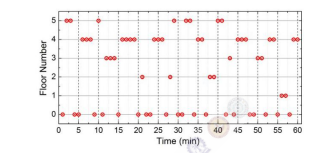
\includegraphics[width=0.5\linewidth]{figs/fig1.png}
    \caption{}
    \label{fig:fig1}
\end{figure}

Which of the following statements are correct?

\begin{enumerate}
    \item The elevator never moves directly from any non-ground floor to another non-ground floor over the one hour period.
    \item The elevator stays on the fourth floor for the longest duration over the one hour period.
\end{enumerate}

\begin{multicols}{2}
\begin{enumerate}
    \item Only i
    \item Only ii
    \item Both i and ii
    \item Neither i nor ii
\end{enumerate}
\end{multicols}
\item Which processing technique is best suited for manufacturing decorative PVC floor tiles?  
\hfill [GATE 2017 XE]

\begin{multicols}{2}
\begin{enumerate}
    \item Blow molding
    \item Filament winding
    \item Rotational molding
    \item Calendering
\end{enumerate}
\end{multicols}

% Q36
\item During deformation of a semi-crystalline polymer, with spherulitic morphology, stressed in tension, what happens to the amorphous and the crystalline regions at the later stages?  
\hfill [GATE 2017 XE]

\begin{multicols}{2}
\begin{enumerate}
    \item Amorphous regions remain intact and only crystallites experience bending and stretching of chains
    \item Only amorphous regions elongate in the stress direction and crystallites remain intact
    \item Amorphous regions elongate in the stress direction and crystallites experience bending and stretching of chains
    \item None of the above
\end{enumerate}
\end{multicols}

% Q37
\item Which of the following statement(s) is / are true regarding the structure-property correlation in polymers?  
\begin{enumerate}
    \item[(i)] Polymers that are less coiled are more crystalline than those that are more coiled  
    \item[(ii)] Branched polymers are more crystalline than the linear ones  
    \item[(iii)] Polymers with inter-chain interactions have higher glass transition temperature than those without inter-chain interactions  
    \item[(iv)] Polymers with inter-chain interactions are more crystalline than those without inter-chain interactions  
\end{enumerate}
\hfill [GATE 2017 XE]

\begin{multicols}{2}
\begin{enumerate}
    \item (i) and (ii)
    \item (ii) and (iii)
    \item (iii) and (iv)
    \item (i) and (iii)
\end{enumerate}
\end{multicols}

% Q38
\item The contrast obtained in scanning electron microscope using back scattered electrons depends on  
\hfill [GATE 2017 XE]

\begin{multicols}{2}
\begin{enumerate}
    \item Atomic number of the specimen material
    \item Accelerating voltage of the microscope
    \item Working distance in the microscope
    \item Type of the electron emitter in the microscope
\end{enumerate}
\end{multicols}
\item Ceramic materials fail at stresses much lower than their theoretical strength due to  
\hfill [GATE 2017 XE]

\begin{multicols}{2}
\begin{enumerate}
    \item Presence of dislocations
    \item High elastic modulus
    \item Presence of voids
    \item Anisotropy in crystal structure
\end{enumerate}
\end{multicols}

% Q41
\item The Miller indices of the first three Bragg peaks in the X-ray diffraction pattern obtained from a polycrystalline iron sample at room temperature are  
\hfill [GATE 2017 XE]

\begin{multicols}{2}
\begin{enumerate}
    \item (111), (200), (220)
    \item (100), (110), (111)
    \item (100), (110), (200)
    \item (110), (200), (220)
\end{enumerate}
\end{multicols}

% Q42
\item The number of close packed planes in the lattice of an FCC metal is  
\hfill [GATE 2017 XE]

\begin{multicols}{2}
\begin{enumerate}
    \item 2
    \item 4
    \item 6
    \item 12
\end{enumerate}
\end{multicols}

% Q43
\item Which of the following treatment(s) can increase the electrical conductivity of silicon  
\begin{enumerate}
    \item[(i)] Heating  
    \item[(ii)] Doping with arsenic  
    \item[(iii)] Doping with aluminium  
    \item[(iv)] Exposure to light  
\end{enumerate}
\hfill [GATE 2017 XE]

\begin{multicols}{2}
\begin{enumerate}
    \item Only (i)
    \item Only (i) and (ii)
    \item Only (ii), (iii) and (iv)
    \item All (i), (ii), (iii) and (iv)
\end{enumerate}
\end{multicols}
\item The unit cell volume of polyethylene (PE) is 0.0933 nm$^3$. Assuming two ethylene repeat units are
contained within each unit cell, the density of a totally crystalline PE will be \underline{\hspace{2cm}} g/cm$^3$.  

(Take the atomic weights for carbon and hydrogen as 12.01 g/mol and 1.008 g/mol, respectively and
the Avogadro’s number as $6.023 \times 10^{23}$ repeat units/mol)  
\hfill [GATE 2017 XE]

\item A continuous, aligned carbon fibre (CF) reinforced polymer composite with 30 vol\% of CF and rest resin was designed for a specific application. The modulus of elasticity of CF is 170 GPa and that of the resin is 3.0 GPa. The modulus of elasticity for this composite in the direction of fibre alignment is \underline{\hspace{2cm}} GPa.  
\hfill [GATE 2017 XE]

% Q45
\item Match the composites in Column I with the most suitable application in Column II  
\hfill [GATE 2017 XE]

\begin{tabular}{ll}
\textbf{Column I} & \textbf{Column II} \\
(P) Exfoliated silicates filled butyl rubber & (1) Automobile pistons \\
(Q) Fiber reinforced aluminium alloy & (2) Contact lenses \\
(R) Silicon carbide whiskers reinforced alumina & (3) Ski boards \\
(S) Carbon particles reinforced plastic composites & (4) Tennis balls \\
& (5) Cutting tools inserts for machining \\
\end{tabular}

\begin{multicols}{2}
\begin{enumerate}
    \item P-4; Q-1; R-5; S-3
    \item P-2; Q-3; R-4; S-5
    \item P-3; Q-5; R-2; S-1
    \item P-2; Q-1; R-5; S-3
\end{enumerate}
\end{multicols}


% Q46
\item Match the processes in Column I with products in Column II  
\hfill [GATE 2017 XE]

\begin{tabular}{ll}
\textbf{Column I} & \textbf{Column II} \\
(P) Slip casting & (1) Metal powders \\
(Q) Zone refining & (2) Thin films \\
(R) Sputtering & (3) Ceramic parts \\
(S) Atomization & (4) Single crystal \\
& (5) Metal sheets \\
\end{tabular}

\begin{multicols}{2}
\begin{enumerate}
    \item P-3; Q-4; R-2; S-1
    \item P-2; Q-1; R-2; S-5
    \item P-3; Q-4; R-5; S-1
    \item P-2; Q-4; R-1; S-5
\end{enumerate}
\end{multicols}

% Q47
\item The value of diffusivity (D) for the diffusion of carbon (C) in $\gamma$-iron at 727$^\degree$C is \underline{\hspace{2cm}} $\times 10^{-13}$ m$^2$/s.(Given $D_{o}=2\times10^{-5}\text{ m}^{2}/\text{s}$, activation energy $Q=142\text{ kJ/mol}$; $R=8.314\text{ J/mol}\cdot\text{ K}$). 

\hfill [GATE 2017 XE]

 \item Refer to the figure below:\\
%pic
\begin{figure}[H]
    \centering
    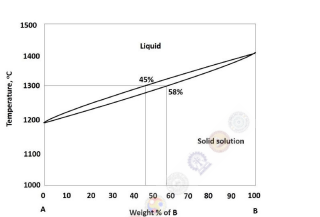
\includegraphics[width=0.5\linewidth]{figs/fig9.png}
    \caption{}
    \label{fig:fig9}
\end{figure}

If the alloy contains 47 wt. \% of A and 53 wt.\% of B at 1300 $^\degree$C, the wt.\% of liquid present in the alloy at this temperature will be \ldots
\hfill [GATE 2017 XE]

\item Which of the following statement(s) is/are true  
\begin{enumerate}
    \item[(i)] All piezoelectric materials are necessarily ferroelectric  
    \item[(ii)] All ferroelectric materials are necessarily piezoelectric  
    \item[(iii)] All pyroelectric materials are necessarily piezoelectric  
    \item[(iv)] All pyroelectric materials are necessarily ferroelectric  
\end{enumerate}
\hfill [GATE 2017 XE]

\begin{multicols}{2}
\begin{enumerate}
    \item (i) and (ii)
    \item (ii) and (iii)
    \item (iii) and (iv)
    \item (ii) and (iv)
\end{enumerate}
\end{multicols}

% Q50
\item If the energy of formation of vacancies in pure copper is 0.9 eV, the fraction of vacancies in pure copper at 27$^\degree$C will be \underline{\hspace{2cm}} $\times 10^{-6}$ (Boltzmann’s constant is $8.62 \times 10^{-5}$ eV/K).  
\hfill [GATE 2017 XE]

% Q51
\item A ceramic material with a critical flaw size of 30 $\mu$m has fracture stress of 300 MPa. For the same material the fracture stress for a critical flaw size of 90 $\mu$m will be \underline{\hspace{2cm}} MPa.  
\hfill [GATE 2017 XE]

% Q52
\item An inorganic material that is transparent under solar light appears coloured when doped with transition metal ions. The possible reason(s) for the colour is/are  
\begin{enumerate}
    \item[(i)] The electronic energy levels of the host material changes significantly by doping  
    \item[(ii)] The doped element selectively absorbs certain wavelength of light other than the band gap absorption  
    \item[(iii)] The doped element emits radiation of specific wavelength  
\end{enumerate}
\hfill [GATE 2017 XE]\\
 which of the statement is correct
\begin{multicols}{2}
\begin{enumerate}
    \item Only (i)
    \item Both (i) and (ii)
    \item Both (ii) and (iii)
    \item Both (i) and (iii)
\end{enumerate}
\end{multicols}

% Q53
\item Copper is an FCC metal with lattice parameter of 3.62 Å. Hall effect measurement shows electron mobility to be $3.2 \times 10^{-2}$ m$^2$/V-s. Electrical resistivity of copper is $1.7 \times 10^{-8}$ $\Omega$m. The electron mean free path in copper at room temperature (300 K) is \underline{\hspace{2cm}} nm. (Take electronic charge as $1.6 \times 10^{-19}$ C)  
\hfill [GATE 2017 XE]

\item In an ionic solid the cation and the anion have ionic radii as 0.8 Å and 1.6 Å respectively. The maximum coordination number of the cation in the structure will be
\hfill [GATE 2017 XE]
\begin{multicols}{2}
\begin{enumerate}
    \item 3
    \item 4
    \item 6
    \item 8
\end{enumerate}
\end{multicols}




\item Which of the following statement(s) is / are true regarding susceptibility of a material
\hfill [GATE 2017 XE]
\begin{enumerate}[label=(\roman*)]
    \item Magnetic susceptibility is positive for a diamagnetic material
    \item Magnetic susceptibility is negative for a diamagnetic material
    \item Magnetic susceptibility is negative for an antiferromagnetic material
    \item Magnetic susceptibility is positive for a paramagnetic material
\end{enumerate}

\begin{multicols}{2}
\begin{enumerate}
    \item (ii) and (iv)
    \item (i) and (iii)
    \item (ii) and (iii)
    \item (i) and (iv)
\end{enumerate}
\end{multicols}
\item In the truss shown, a mass $m=10\text{kg}$ is hung from the node J. The magnitude of net force (in Newtons) transferred by the truss $\underline{\text{EFGHIJ}}$ onto the truss $\underline{\text{JKLMNO}}$ at the node J is $\underline{\hspace{2cm}}$.
Assume acceleration due to gravity, $g=10\text{m/s}^2$.
\hfill [GATE 2017 XE]
%pic
\begin{figure}[H]
    \centering
    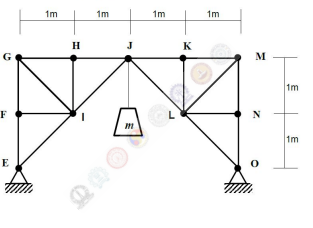
\includegraphics[width=0.5\linewidth]{figs/fig10.png}
    \caption{}
    \label{fig:fig10}
\end{figure}
\item A ball moves along a planar frictionless slot as shown. Which one of the paths shown closely matches the path taken by the ball after it exits the slot at E?
\begin{figure}[H]
    \centering
    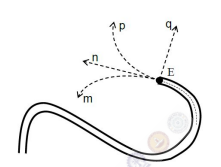
\includegraphics[width=0.5\linewidth]{figs/fig11.png}
    \caption{}
    \label{fig:fig11}
\end{figure}
\hfill [GATE 2017 XE]
%[pic]

\item A rod EF moving in a plane has velocity $V_E$ at E and $V_F$ at F that are parallel to each other. Which of the following CANNOT be true?  

\hfill [GATE 2017 XE]

\begin{figure}[H]
    \centering
    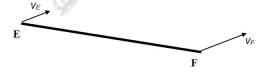
\includegraphics[width=0.5\linewidth]{figs/fig12.png}
    \caption{}
    \label{fig:fig12}
\end{figure}

\begin{multicols}{2}
\begin{enumerate}
    \item Both $V_E$ and $V_F$ are perpendicular to EF.  
    \item Magnitude of $V_E$ is equal to the magnitude of $V_F$ and the angular velocity of EF is zero.  
    \item The velocity $V_E$ is not perpendicular to EF and the angular velocity of EF is nonzero.  
    \item Magnitude of $V_E$ is not equal to the magnitude of $V_F$ and the angular velocity of EF is nonzero.  
\end{enumerate}
\end{multicols}

% Q59
\item The beam shown below carries two external moments. A counterclockwise moment of magnitude $2M$ acts at point B and a clockwise moment of magnitude $M$ acts at the free end C. The beam is fixed at A. The shear force at a section close to the fixed end is equal to \underline{\hspace{2cm}}.  

\hfill [GATE 2017 XE]

\begin{figure}[H]
    \centering
    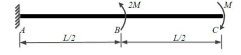
\includegraphics[width=0.5\linewidth]{figs/fig13.png}
    \caption{}
    \label{fig:fig13}
\end{figure}

\begin{multicols}{2}
\begin{enumerate}
    \item $\dfrac{2M}{L}$  
    \item $\dfrac{M}{L}$  
    \item $0$  
    \item $\dfrac{M}{2L}$  
\end{enumerate}
\end{multicols}

% Q60
\item Two pendulums are shown below. Pendulum-A carries a bob of mass $m$, hung using a hinged massless rigid rod of length $L$, whereas Pendulum-B carries a bob of mass $4m$ and length $\dfrac{L}{4}$. The ratio of natural frequencies of Pendulum-A and Pendulum-B is given by \underline{\hspace{2cm}}.

\hfill [GATE 2017 XE]

\begin{figure}[H]
    \centering
    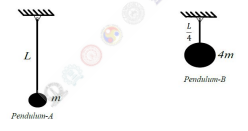
\includegraphics[width=0.5\linewidth]{figs/fig14.png}
    \caption{}
    \label{fig:fig14}
\end{figure}
\begin{multicols}{2}
\begin{enumerate}
    \item 1 : 2  
    \item 1 : 1  
    \item $\sqrt{2}$ : 1  
    \item 2 : 1  
\end{enumerate}
\end{multicols}
\item A closed thin-walled cylindrical steel pressure vessel of wall thickness $t=1\text{mm}$ is subjected to internal pressure. The maximum value of pressure $p$ (in kPa) that the wall can withstand based on the maximum shear stress failure theory is given by (Yield strength of steel is $200\text{MPa}$ and mean radius of the cylinder $r = 1\text{m}$).\hfill [GATE 2017 XE]

\begin{multicols}{4}
\begin{enumerate}
    \item 100
    \item 200
    \item 300
    \item 400
\end{enumerate}
\end{multicols}



\item The state of stress at a point in a body is represented using components of stresses along X and Y directions as shown. Which one of the following represents the state of stress along X' and Y' axes? (X' - axis is at 45\textdegree{} clockwise with respect to X - axis).

\hfill [GATE 2017 XE]

\begin{figure}[H]
    \centering
    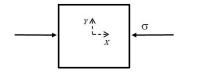
\includegraphics[width=0.5\linewidth]{figs/fig15.png}
    \caption{}
    \label{fig:fig15}
\end{figure}

\begin{figure}[H]
    \centering
    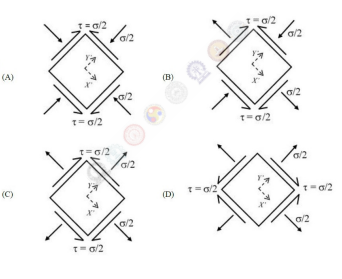
\includegraphics[width=0.5\linewidth]{figs/fig16.png}
    \caption{}
    \label{fig:placeholder}
\end{figure}

\item An aluminum specimen with an initial gauge diameter $d_0 = 10\text{mm}$ and a gauge length $l_0 = 100\text{mm}$ is subjected to tension test. A tensile force $P = 50\text{kN}$ is applied at the ends of the specimen as shown resulting in an elongation of $1\text{mm}$ in the gauge length. The Poisson's ratio $(\nu)$ of the specimen is
\underline{\hspace{2cm}}
Shear modulus of the material $G = 25\text{GPa}$. Consider engineering stress-strain conditions.

\hfill [GATE 2017 XE]

\begin{figure}[H]
    \centering
    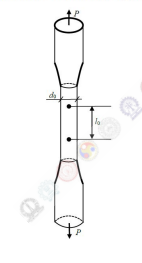
\includegraphics[width=0.5\linewidth]{figs/fig17.png}
    \caption{}
    \label{fig:placeholder}
\end{figure}
\item A rectangular sheet $ABCD$ of dimensions $a$ and $b$ along X and Y directions, respectively, is stretched to a rectangle $AB'C'D'$, as shown. The maximum principal strain $(\epsilon_1)$ and minimum principal strain $(\epsilon_2)$ due to the stretch are given by

\hfill [GATE 2017 XE]

\begin{figure}[H]
    \centering
    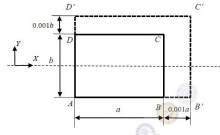
\includegraphics[width=0.5\linewidth]{figs/fig18.png}
    \caption{}
    \label{fig:placeholder}
\end{figure}

\begin{multicols}{2}
    \begin{enumerate}
        \item[(A)] $0.001$ and $0.001$
        \item[(B)] $-0.001$ and $0.001$
        \item[(C)] $-0.001$ and $-0.001$
        \item[(D)] $-0.001$ and $0.001$
    \end{enumerate}
\end{multicols}


\item A solid bar of uniform square cross-section of side $b$ and length $L$ is rigidly fixed to the supports at the two ends. When the temperature in the rod is increased uniformly by $T_c$, the bar undergoes elastic buckling. Assume Young's modulus $E$ and coefficient of thermal expansion $\alpha$ to be independent of temperature. The coefficient of thermal expansion $\alpha$ is given by
\hfill [GATE 2017 XE]

\begin{multicols}{2}
    \begin{enumerate}
        \item[(A)] $\dfrac{3\pi^2 b^2}{E T_c L^2}$
        \item[(B)] $\dfrac{\pi^2 b^2}{T_c L^2}$
        \item[(C)] $\dfrac{\pi^2 b^2}{2 T_c L^2}$
        \item[(D)] $\dfrac{3T_c}{2b L^2}$
    \end{enumerate}
\end{multicols}



\item Two rigid blocks, of masses $10\text{kg}$ and $15\text{kg}$, are arranged one on top of the other and placed on a horizontal rough surface as shown. The blocks are connected to each other through an inextensible cable passing over a frictionless pulley. The coefficients of static friction between the blocks and also between the bottom block and the surface are all equal to $0.3$. The force $P$ (in Newtons) needed to set the blocks in motion towards right is
(Assume acceleration due to gravity $g = 10 \text{m/s}^2$)

\hfill [GATE 2017 XE]

\begin{figure}[H]
    \centering
    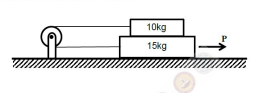
\includegraphics[width=0.5\linewidth]{figs/fig19.png}
    \caption{}
    \label{fig:placeholder}
\end{figure}
\item A truss system EFGH shown below is built using members EF, GH and FH of the same cross-sectional area $10\text{mm}^2$ and member FG of cross-sectional area $20\text{mm}^2$. The total strain energy stored (in Nm) in the system due to a force $P=1\text{kN}$ acting at F is $\underline{\hspace{2cm}}$

Assume elastic deformations and members are made of steel with elastic modulus of $200\text{GPa}$.
$1\text{m}$

\hfill [GATE 2017 XE]

\begin{figure}[H]
    \centering
    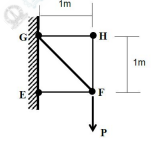
\includegraphics[width=0.5\linewidth]{figs/fig20.png}
    \caption{}
    \label{fig:placeholder}
\end{figure}

\item A rigid frame grips on to a steel wall as shown using a powerful magnet at the top support G and with a roller support at E. EF is horizontal. A man stands on the platform attached to the frame 1m away from the wall as shown. Assume the frame and magnet assembly to be of negligible weight and the mass of the man to be 80kg. The magnitude of the reaction (in Newtons) exerted by the frame onto the steel wall due to the weight of the man is $\underline{\hspace{2cm}}$
The magnetic force of attraction of the magnet at no load condition is 1kN. Magnet can be assumed to be small enough that it offers negligible moment resistance. Assume acceleration due to gravity, g=10m/s$^{2}$.

\hfill [GATE 2017 XE]

\begin{figure}[H]
    \centering
    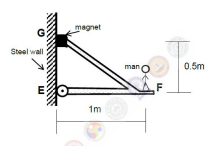
\includegraphics[width=0.5\linewidth]{figs/fig21.png}
    \caption{}
    \label{fig:placeholder}
\end{figure}
\item A manually operated band brake has a control lever EFG as shown and has a coefficient of kinetic friction equal to 0.2. The cylinder initially rotates clockwise at a constant frequency of 10 revolutions per second. A force P=300N is applied at G. The pin support at O is frictionless. The radius of the cylinder $r=0.15\text{m}$ and the radius of gyration is $0.1\text{m}$. The mass of the cylinder is $50\text{kg}$. Assume acceleration due to gravity $g=10\text{m/s}^2$. The time required (in seconds) to reduce the rotational frequency to 5 revolutions per second is $\underline{\hspace{2cm}}$

\hfill [GATE 2017 XE]

\begin{figure}[H]
    \centering
    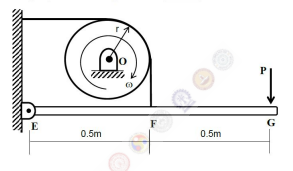
\includegraphics[width=0.5\linewidth]{figs/fig22.png}
    \caption{}
    \label{fig:placeholder}
\end{figure}
\item In a pin-connected mechanism shown, load P applied at F is 50N. Neglect the weight of the links and assume $k=\text{1kN/m}$ for the spring. The bars EH and FG are pinned at O at their centre such that the lengths of EO, GO, HO and FO are all equal to $l=\text{0.2m}$. The spring between G and H is unstretched when $\theta=45^{\degree}$.
The angle $\theta$ (in degrees) under equilibrium is \underline{\hspace{2cm}}

\hfill [GATE 2017 XE]

\begin{figure}[H]
    \centering
    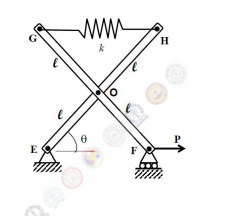
\includegraphics[width=0.5\linewidth]{figs/fig23.png}
    \caption{}
    \label{fig:placeholder}
\end{figure}

\item The frame shown below carries a vertical load $P=10\text{kN}$ at its free end $\underline{D}$. The frame is fixed at $\underline{A}$ and has a roller support at $\underline{B}$. Magnitude of the reaction force at $\underline{B}$ (in $\text{kN}$) is $\underline{\hspace{2cm}}$.

Assume that the effect of the axial force on bending is negligible.

\hfill [GATE 2017 XE]

\begin{figure}[H]
    \centering
    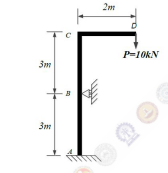
\includegraphics[width=0.5\linewidth]{figs/fig24.png}
    \caption{}
    \label{fig:placeholder}
\end{figure}

\item Consider the system shown below. Mass $M$ is fixed to the rod $AC$ at a distance $x$ from the hinge point at $B$. Two springs of stiffness $3K$ and $K$ are attached to the rod at points $A$ and $C$, respectively. The natural frequency of angular oscillation of the system about $B$ is $20 \text{ rad/s}$. Assume the rod to be rigid and massless. Magnitude of $x$ (in metres) is \_\_\_\_\_\_ ($M=30\text{kg}$ and $K=1\text{kN/m}$).

\hfill [GATE 2017 XE]

\begin{figure}[H]
    \centering
    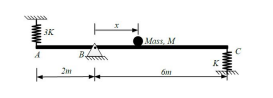
\includegraphics[width=0.5\linewidth]{figs/fig25.png}
    \caption{}
    \label{fig:placeholder}
\end{figure}

\item The simply supported beam shown below is subjected to a clockwise moment $M$ at point $A$ and two counterclockwise moments $2M$ and $M$ at points $B$ and $C$, respectively. Which one of the following is the correct bending moment diagram (tensile at bottom is positive moment) for the beam?

\begin{figure}[H]
    \centering
    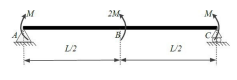
\includegraphics[width=0.5\linewidth]{figs/fig26.png}
    \caption{}
    \label{fig:placeholder}
\end{figure}

\hfill [GATE 2017 XE]

\begin{figure}[H]
    \centering
    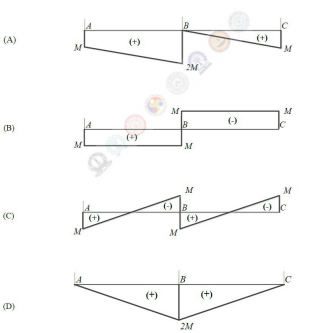
\includegraphics[width=0.5\linewidth]{figs/fig27.png}
    \caption{}
    \label{fig:placeholder}
\end{figure}

\item The structure shown below is of rectangular cross section and carries a load of 10kN at its free end E. Maximum bending stress (in MPa) developed in the beam due the external load is\underline{\hspace{2cm}} The depth of the beam is 300mm and the width is 150mm

\hfill [GATE 2017 XE]

\begin{figure}[H]
    \centering
    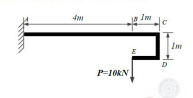
\includegraphics[width=0.5\linewidth]{figs/fig28.png}
    \caption{}
    \label{fig:placeholder}
\end{figure}

\item Two circular rods shown below carry the same axial load $P$. The Rod-A has uniform cross-section and the Rod-B has non-uniform cross-section as shown. The ratio of elongation of Rod-A to Rod-B is given by

\hfill [GATE 2017 XE]

\begin{figure}[H]
    \centering
    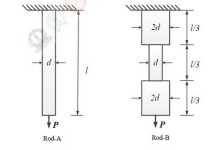
\includegraphics[width=0.5\linewidth]{figs/fig29.png}
    \caption{}
    \label{fig:placeholder}
\end{figure}
%pic 
\begin{multicols}{2}
\begin{enumerate}
    \item 1:1
    \item 1:2
    \item 2:1
    \item 3:1
\end{enumerate}
\end{multicols}
\item A composite shaft is made of a steel tube with an inner brass core perfectly bonded together as shown. The shaft is fixed at one end and subjected to a torque of $2T$ at the other end. Shear modulus of steel is $G$ and that of brass is $G/2$. The outer radius of the steel tube is $R=2r$ and radius of the inner brass core is $r$. The magnitude of shear stress at the interface (point X) and in the steel tube is closest to

\hfill [GATE 2017 XE]

\begin{figure}[H]
    \centering
    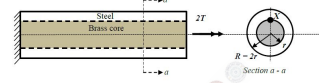
\includegraphics[width=0.5\linewidth]{figs/fig30.png}
    \caption{}
    \label{fig:placeholder}
\end{figure}

\begin{multicols}{4}
\begin{enumerate}
    \item $0.041\frac{T}{r^{3}}$
    \item $0.082\frac{T}{r^{3}}$
    \item $0.16\frac{T}{r^{3}}$
    \item $0.41\frac{T}{r^{3}}$
\end{enumerate}
\end{multicols}
\item A massless rod of rectangular cross-section is subjected to a force $P$ at origin $O$ as shown. The expression for the stress $\sigma_{zz}$ at point $Q$ is given by

\hfill [GATE 2017 XE]

\begin{figure}[H]
    \centering
    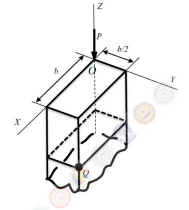
\includegraphics[width=0.5\linewidth]{figs/fig31.png}
    \caption{}
    \label{fig:placeholder}
\end{figure}

\begin{enumerate}
    \begin{multicols}{2}
        \item[(A)] $\frac{6P}{b^2}$
        \item[(B)] $\frac{10P}{b^2}$
        \item[(C)] $-\frac{14P}{b^2}$
        \item[(D)] $-\frac{P}{b^2}$
    \end{multicols}
\end{enumerate}

\item Given $d\phi = f(T)dT + (T/V)dV$ and $d\psi = Tdp + (T/p^{2})dV$, then  

\hfill [XE GATE 2017]

\begin{enumerate}
\begin{multicols}{2}
\item Both $\phi$ and $\psi$ are properties
\item Neither $\phi$ nor $\psi$ is a property
\item $\phi$ is a property but $\psi$ is not a property
\item $\psi$ is a property but $\phi$ is not a property
\end{multicols}
\end{enumerate}


\item A paddle wheel is installed in a rigid insulated tank containing 10 kg air ($C_v = 0.718 \, kJ/kg.K$). A torque of 100 N.m is applied on the paddle wheel to rotate it at 60 revolutions per minute for 2 minutes. At the end of the process, the increase in temperature of air in $^\circ$C is  

\hfill [XE GATE 2017]

\begin{enumerate}
\begin{multicols}{2}
\item 0  
\item 5.25  
\item 10.50  
\item 21.50  
\end{multicols}
\end{enumerate}


\item Consider two systems each containing 20 kg of air at the same temperature and pressure. It is desired to increase the temperature of the air in both systems by 10$^\circ$C. One system undergoes a constant pressure heat addition process and the other undergoes a constant volume heat addition process. The difference in the values of heat transferred to the two systems in kJ is  

\hfill [XE GATE 2017]

\begin{enumerate}
\begin{multicols}{2}
\item 30.5  
\item 144.2  
\item 57.5  
\item 73.2  
\end{multicols}
\end{enumerate}


\item A refrigerator is used to maintain certain space at 10$^\circ$C. It pumps 18000 kJ/hour of heat from the space to the atmosphere at 30$^\circ$C. If the power input to the refrigerator is 2 kW, the ratio of COP of this refrigerator to that of a Carnot refrigerator (up to 2 decimal places) is  

\hfill [XE GATE 2017]


\item A thermal cycle receives 2000 kJ of heat from a heat source at 1000 K. It rejects 300 kJ of heat to a heat sink at 300 K and also rejects 250 kJ of heat to another heat sink at 200 K during the cycle. The cycle is  

\hfill [XE GATE 2017]

\begin{enumerate}
\begin{multicols}{2}
\item reversible  
\item irreversible  
\item impossible  
\item work absorbing  
\end{multicols}
\end{enumerate}


\item Saturated liquid water is slowly heated at a constant pressure of 200 kPa to a final state where its quality reaches 0.65. For water at 200 kPa: $T_{sat} = 120.23^\circ$C, $h_f = 504.68$ kJ/kg, $h_{fg} = 2706.60$ kJ/kg. The increase in specific entropy in kJ/kg.K is  

\hfill [XE GATE 2017]

\begin{enumerate}
\begin{multicols}{2}
\item 3.44  
\item 3.64  
\item 3.84  
\item 4.04  
\end{multicols}
\end{enumerate}
\item Given the thermodynamic functional relations: $p = p(v,T)$ and $T = T(p,v)$, the term  
\begin{align}
    \left( \frac{\partial^2 v}{\partial T \partial p} \right)
\end{align}
is equal to  

\hfill [XE GATE 2017]

\begin{enumerate}
\begin{multicols}{2}
\item $\left( \frac{\partial T}{\partial v} \right)_{p}$  
\item $\left( \frac{\partial T}{\partial p} \right)_{v}$  
\item $\left( \frac{\partial T}{\partial v} \right)_{T}$  
\item 1  
\end{multicols}
\end{enumerate}


\item Two closed cycle gas turbine engines, A and B, operate on air standard Brayton cycle with efficiencies of $\eta_A$ and $\eta_B$, respectively. If they operate between the same maximum and minimum temperatures, but with different pressure ratios of $r_{pA}$ and $r_{pB}$ ($r_{pA} > r_{pB}$), then  

\hfill [XE GATE 2017]

\begin{enumerate}
\begin{multicols}{2}
\item $\eta_A > \eta_B$  
\item $\eta_A < \eta_B$  
\item $\eta_A = \eta_B$  
\item Cannot be determined as the efficiencies are maximum only at the optimal $r_p$ values.  
\end{multicols}
\end{enumerate}


\item The values of density and isentropic compressibility of water at certain pressure and temperature are given as 1000 kg/m$^3$ and $4 \times 10^{-10}$ Pa$^{-1}$, respectively. The speed at which sound travels in water under these conditions in m/s is equal to  

\hfill [XE GATE 2017]


\item Length of a certain metal rod at 0$^\circ$C is 10 cm. The coefficient of linear expansion of that metal varies with temperature as $10^{-4} + 10^{-7}T$ (cm/cm)/$^\circ$C. When the length of the metal rod is 10.2 cm, the rise in temperature in $^\circ$C is  

\hfill [XE GATE 2017]


\item In a polytropic compression process, one kg of an ideal gas having a molecular weight of 40 kg/kmol is compressed from 100 kPa, 300 K to 400 kPa, 360 K. The magnitude of the work in kJ for the process is  

\hfill [XE GATE 2017]

\begin{enumerate}
\begin{multicols}{2}
\item 52.3  
\item 62.3  
\item 72.3  
\item 82.3  
\end{multicols}
\end{enumerate}
\item Two streams of air ($C_p = 1005 \text{ J/kg.K}$) flow through insulated pipes 1 and 2 with the conditions as shown in figure. They mix in an insulated pipe-3 and the mixture steadily exits with a velocity of 100 m/s at 150 kPa. Neglecting the change in potential energy in all the pipes, the exit area of the pipe-3 in $\text{m}^2$ (up to 3 decimal places) is \underline{\hspace{2cm}}

\hfill [XE GATE 2017]

\begin{figure}[H]
    \centering
    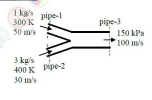
\includegraphics[width=0.5\linewidth]{figs/fig32.png}
    \caption{}
    \label{fig:placeholder}
\end{figure}

\item A 1 m$^3$ rigid vessel contains air at 200 kPa. A vacuum pump is connected to the vessel in order to control the pressure inside. The volume flow rate of air through the pump is maintained at a constant value of 0.1 m$^3$/s. If the pump operates for 10 seconds and the temperature of the air is maintained constant during operation, the pressure in the tank in kPa after 10 seconds (up to 2 decimal places) is  

\hfill [XE GATE 2017]


\item A heat engine receives $Q_1$ kJ of heat from a hot reservoir and rejects $Q_2$ kJ of heat to a cold reservoir. The work delivered by the heat engine is entirely supplied to a heat pump, which receives $Q_3$ kJ of heat from another reservoir and rejects $Q_4$ kJ of heat to the same cold reservoir. If the efficiency of the heat engine is 0.4 and COP of the heat pump is 4.0, the value of $\brak{Q_2 + Q_4}/Q_1$ (up to 1 decimal place) is  

\hfill [XE GATE 2017]


\item A block of ice of mass 2 kg at 0$^\circ$C is dropped into an insulated vessel containing 10 kg of liquid water at 25$^\circ$C. The latent heat of melting of ice is 330 kJ/kg and specific heat of water is 4.2 kJ/kg.K. The change in the entropy of the universe in kJ/K (up to 3 decimal places) is  

\hfill [XE GATE 2017]


\item A pure substance ($C_v = 0.733$ kJ/kg.K) undergoes a reversible process in which its temperature increases linearly from 40$^\circ$C to 85$^\circ$C and its specific entropy increases by 600 J/kg.K. The work done by the system in kJ/kg is  

\hfill [XE GATE 2017]

\begin{enumerate}
\begin{multicols}{2}
\item \brak{160.2}  
\item \brak{164.3}  
\item \brak{168.3}  
\item \brak{172.3}  
\end{multicols}
\end{enumerate}


\item An ideal gas having a mass of 0.5 kg is initially at 300 kPa, 80$^\circ$C and occupies a volume of 0.14 m$^3$. The gas undergoes an adiabatic process, where 50 kJ of work is transferred to the gas. The pressure and temperature at the final state are 300 kPa and 0.20 m$^3$. The change in the entropy of the gas in kJ/K is  

\hfill [XE GATE 2017]

\begin{enumerate}
\begin{multicols}{2}
\item \brak{160.3}  
\item \brak{175.3}  
\item \brak{190.3}  
\item \brak{195.3}  
\end{multicols}
\end{enumerate}


\item The van der Waals equation of state is given as,  
\begin{align}
    \left( p + \frac{a}{v^2} \right)(v-b) = RT,
\end{align} 
where p in bar, v in m$^3$/kmol and T is in K.  

For air, the constants, a and b, are 1.358 (bar m$^6$/kmol$^2$) and 0.0367 (m$^3$/kmol), respectively. Air is contained in a system at 160 K and 0.08 m$^3$/kmol. If the pressure calculated using ideal gas equation is p$_i$ and the pressure calculated using van der Waals equation of state, then p$_i$/p$_{vdw}$ is equal to \underline{\hspace{2cm}}.  

\hfill [XE GATE 2017]

\begin{enumerate}
\begin{multicols}{2}
\item 1.78  
\item 1.52  
\item 1.28  
\item 1.04  
\end{multicols}
\end{enumerate}


\item The values of specific volume of H$_2$O at 100$^\circ$C for saturated liquid and saturated vapor states are 0.00104 m$^3$/kg and 1.673 m$^3$/kg, respectively. The slope of saturation pressure versus temperature curve, $\left(\frac{dp_{sat}}{dT}\right)_{sat}$ is 3570 kPa/K. The change in enthalpy in kJ/kg between the two saturation states is \underline{\hspace{2cm}}.  

\hfill [XE GATE 2017]


\item In a steam power plant, steam is first expanded isentropically in a turbine from an initial condition of 100 bar and 500 $^\circ$C to a pressure of 40 bar. Then the steam is reheated up to 500 $^\circ$C at constant pressure. The steam is then expanded isentropically in another turbine up to a condenser pressure 0.01 bar. For steam, at 100 bar, 500$^\circ$C: $h=3373.7$ kJ/kg, $s = 6.5966$ kJ/kg.K: at 40 bar, 500$^\circ$C: $h = 3445.3$ kJ/kg, $s = 7.0901$ kJ/kg.K and at 0.01 bar: $h_{f}=29.3$ kJ/kg. $h_{g}=2514.2$ kJ/kg. $s_{f}=0.1059$ kJ/kg.K. $s_{g} = 8.9756$ kJ/kg.K. The dryness fraction at the condenser inlet (up to 2 decimal places) is   \underline{\hspace{2cm}}.

\hfill [XE GATE 2017]


\item Air contains by volume 79\% N$_2$ (molecular weight = 28 kg/kmol) and 21\% O$_2$ (molecular weight = 32 kg/kmol). A stream of air flows at 32$^\circ$C, 1 bar, at a rate of 2 kmol/s and is mixed with another stream of pure O$_2$ flowing at 0.4 kmol/s. The molecular weight of the mixture (up to 2 decimal places) is \underline{\hspace{2cm}}.  

\hfill [XE GATE 2017]


\item Moist air enters a duct at a rate of 3 kg/s at 10$^\circ$C, 80\% relative humidity. The air is heated as it flows through the duct and exits at 30$^\circ$C. No moisture is added or removed and the pressure of air in the duct is constant at 1 bar. The saturation vapor pressure ($p_v$) of H$_2$O at 10$^\circ$C is 0.01228 bar. Specific enthalpy values of dry air at inlet and outlet of the duct are respectively 283.1 kJ/kg and 303.2 kJ/kg. The corresponding specific enthalpy values for water vapor are 2519.8 kJ/kg and 2556.3 kJ/kg. For steady state operation the amount of heat added to the moist air in kW (up to 2 decimal places) is \underline{\hspace{2cm}}.  

\hfill [XE GATE 2017]
\item Poly(ethylene terephthalate) is synthesized from  

\hfill [GATE XE 2017]  

\begin{multicols}{2}  
\begin{enumerate}  
\item Ethylene + dimethyl terephthalate  
\item Ethylene + terephthalic acid  
\item Glycerol + terephthalic acid  
\item Ethylene Glycol + terephthalic acid  
\end{enumerate}  
\end{multicols}  

\item Poly(vinyl chloride) has a higher T$_g$ than polypropylene due to the presence of  

\hfill [GATE XE 2017]  

\begin{multicols}{2}  
\begin{enumerate}  
\item Bulky side groups  
\item Polar interactions  
\item Restriction of bond rotation  
\item Non-polar interactions  
\end{enumerate}  
\end{multicols}  

\item The filler which would impart electrical conductivity to a polymer is  

\hfill [GATE XE 2017]  

\begin{multicols}{2}  
\begin{enumerate}  
\item Carbon black  
\item Talc  
\item Glass beads  
\item Calcium carbonate  
\end{enumerate}  
\end{multicols}  

\item Which one of the following catalysts is used to prepare ‘isotactic’ polypropylene?  

\hfill [GATE XE 2017]  

\begin{multicols}{2}  
\begin{enumerate}  
\item Alkyl lithium  
\item BF$_3$  
\item Ziegler-Natta  
\item AIBN  
\end{enumerate}  
\end{multicols}  

\item Novolac and Resole are A-stage low molecular weight phenolic resin products that are  

\hfill [GATE XE 2017]  

\begin{multicols}{2}  
\begin{enumerate}  
\item Soluble and fusible  
\item Soluble but infusible  
\item Insoluble and fusible  
\item Insoluble and infusible  
\end{enumerate}  
\end{multicols}  

\item Which of the following reagents can act as an initiator at room temperature?  

\hfill [GATE XE 2017]  

\begin{multicols}{2}  
\begin{enumerate}  
\item AIBN  
\item Dicumyl peroxide  
\item Dibenzoyl peroxide  
\item Fe$^{2+}$ + H$_2$O$_2$  
\end{enumerate}  
\end{multicols}  

\item The impact strength of polystyrene can be enhanced by blending/mixing with  

\hfill [GATE XE 2017]  

\begin{multicols}{2}  
\begin{enumerate}  
\item Carbon black  
\item PMMA  
\item Polybutadiene  
\item Glass fibre  
\end{enumerate}  
\end{multicols}  

\item The melt processing temperature of a semicrystalline thermoplastic polymer is  

\hfill [GATE XE 2017]  

\begin{multicols}{2}  
\begin{enumerate}  
\item Between T$_g$ and T$_m$  
\item Equal to T$_m$  
\item Lower than T$_m$  
\item Higher than T$_m$  
\end{enumerate}  
\end{multicols}  

\item The unit of viscosity of a polymer is expressed as  

\hfill [GATE XE 2017]  

\begin{multicols}{2}  
\begin{enumerate}  
\item Pa·s  
\item Pa·s$^{-1}$  
\item Pa·s$^{2}$  
\item Pa·s$^{-3}$  
\end{enumerate}  
\end{multicols}

\item Based on the graphs 1-5, which option best describes the stress-strain behaviour of materials listed as P, Q, R, S and T?

\hfill [GATE XE 2017]  

\begin{figure}[H]
    \centering
    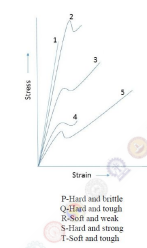
\includegraphics[width=0.5\linewidth]{figs/fig33.png}
    \caption{}
    \label{fig:placeholder}
\end{figure}

\begin{multicols}{2}
\begin{enumerate}
    \item P-2; Q-1; R-5; S-4; T-3
    \item P-1; Q-3; R-4; S-2; T-5
    \item P-1; Q-2; R-5; S-3; T-4
    \item P-2; Q-3; R-1; S-4; T-5
\end{enumerate}
\end{multicols}
\item The two characterization techniques which can be used to determine degree of crystallinity of a polymer are

P. Scanning Electron Microscopy \\
Q. Thermogravimetric Analysis \\
R. Wide Angle X-Ray Diffraction \\
S. Differential Scanning Calorimetry

\hfill [XE GATE 2017]

\begin{multicols}{2}
\begin{enumerate}
\item P\&R
\item Q\&R
\item R\&S
\item Q\&S
\end{enumerate}
\end{multicols}
\item The density of polyethylene crystals is 998 kg m$^{-3}$ and that of totally amorphous polyethylene is 856 kg m$^{-3}$. If the density of a polyethylene sample is 949 kg m$^{-3}$, the crystallinity in volume fraction is \underline{\hspace{2cm}}. (round off final answer to two digits after decimal place).  

\hfill [GATE XE 2017]  

\item The polydispersity index of a polymer sample containing 200 molecules each of molecular weight 10,000 g mol$^{-1}$, 300 molecules each of molecular weight 30,000 g mol$^{-1}$ and 500 molecules each of molecular weight 50,000 g mol$^{-1}$ is \underline{\hspace{2cm}}.. (round off final answer to two digits after decimal place).  

\hfill [GATE XE 2017]  

\item Match the following rubber additives to their function:  

\hfill [GATE XE 2017]  

\begin{tabular}{ll}
\textbf{Additive} & \textbf{Function} \\
P. Dicumyl peroxide & 1. Ultrafast accelerator \\
Q. Pentachlorothiophenol & 2. Activator \\
R. ZnO with stearic acid & 3. Curing agent \\
S. Zinc diethyldithiocarbamate & 4. Peptizer
\end{tabular}

\begin{multicols}{2}  
\begin{enumerate}  
\item P-3; Q-1; R-2; S-4  
\item P-3; Q-1; R-4; S-2  
\item P-3; Q-4; R-2; S-1  
\item P-3; Q-4; R-1; S-2  
\end{enumerate}  
\end{multicols}  

\item A composite of polypropylene reinforced with 20\% by volume of glass fibre is to be prepared. If the density of glass fibre is 2540 kg m$^{-3}$ and polypropylene is 900 kg m$^{-3}$, the melt flow index of this glass fibre composite is \underline{\hspace{2cm}}. g/10 min. (round off final answer to one digit after decimal place).  

\hfill [GATE XE 2017]  

\item Match the following terminology to the appropriate polymer processing technique:

\begin{tabular}{|l|l|}
\hline
\textbf{Terminology} & \textbf{Processing Technique} \\
\hline
P. Die-swell & 1. Two roll mill mixing \\
Q. Breathing & 2. Thermoforming \\
R. Plug-assisted & 3. Extrusion \\
S. Mastication & 4. Compression moulding \\
\hline
\end{tabular}

\hfill [GATE XE 2017] 

\begin{multicols}{2}
\begin{enumerate}
    \item P-1: Q-2: R-3: S-4
    \item P-3: Q-4: R-2: S-1
    \item P-2: Q-3: R-4: S-1
    \item P-2: Q-1: R-4: S-3
\end{enumerate}
\end{multicols}




\item Match the polymer in Column A to its application in Column B:

\begin{tabular}{|l|l|}
\hline
\textbf{Column A} & \textbf{Column B} \\
\hline
P. Nylon & 1. Television cabinet \\
Q. Polyethylene & 2. Tyre \\
R. Cis-1,4-polyisoprene & 3. Mechanical gear \\
S. Acrylonitrile-butadiene-styrene & 4. Packaging \\
\hline
\end{tabular}


\hfill [GATE XE 2017] 

\begin{multicols}{2}
\begin{enumerate}
    \item P-3: Q-4: R-2: S-1
    \item P-4: Q-3: R-2: S-1
    \item P-4: Q-2: R-3: S-1
    \item P-3: Q-4: R-1: S-2
\end{enumerate}
\end{multicols}
\item For the polycondensation of equimolar amounts of adipic acid with hexamethylene diamine, if the number average degree of polymerization is 100, then the extent of reaction is \underline{\hspace{2cm}}

\hfill [GATE XE 2017] 

\item The relaxation time for a rubber band at 23 $^\circ$C is 60 days. If it is stressed to 2 MPa initially, then the time required before the stress relaxes to 1 MPa is \underline{\hspace{2cm}} days (round off final answer to two digits after decimal point).

\hfill [GATE XE 2017] 

\item Match the processing technique in Column A to the corresponding shear rate (s$^{-1}$) in Column B.

\begin{tabular}{|l|l|}
\hline
\textbf{Column A} & \textbf{Column B} \\
\hline
P. Injection Moulding & 1. 1-10 \\
Q. Extrusion & 2. 10-100 \\
R. Calendering & 3. 100-1000 \\
S. Compression Moulding & 4. 1000-10000 \\
\hline
\end{tabular}

\begin{enumerate}
    \item[(A)] P-1; Q-3; R-2; S-4
    \item[(B)] P-4; Q-2; R-3; S-1
    \item[(C)] P-4; Q-3; R-1; S-2
    \item[(D)] P-4; Q-3; R-2; S-1
\end{enumerate}


\item Given $T_g$ of polymer A is 100 $^\circ$C and that of polymer B is -100 $^\circ$C, then the $T_g$ of a miscible blend of A and B containing 30 wt\% of A is \rule{2cm}{0.15mm} $^\circ$C (round off final answer to a single digit after decimal point).

\hfill [GATE XE 2017] 

\item Match plots 1-4 given in the figure below with the correct flow behavior of polymeric fluid listed as P, Q, R \& S.
\begin{figure}[H]
    \centering
    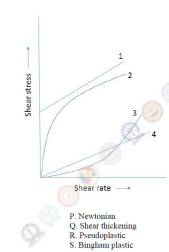
\includegraphics[width=0.5\linewidth]{figs/fig34.png}
    \caption{}
    \label{fig:placeholder}
\end{figure}

\hfill [GATE XE 2017] 

\begin{multicols}{2}
\begin{enumerate}
    \item P-4: Q-2: R-3; S-1
    \item P-4: Q-3: R-3; S-1
    \item P-4; Q-3; R-1; S-2
    \item P-1, Q-3; R-2; S-4
\end{enumerate}
\end{multicols}
\item Indicate the correct group that contains a monosaccharide, a disaccharide and a trisaccharide.

\hfill [XE GATE 2017]

\begin{multicols}{2}
\begin{enumerate}
\item Glucose, sucrose, mannose
\item Ribose, lactose, raffinose
\item Mannose, maltose, lactose
\item Raffinose, stachyose, glucose
\end{enumerate}
\end{multicols}


\item In which of the following products, ‘must’ is used as the substrate for fermentation?

\hfill [XE GATE 2017]

\begin{multicols}{2}
\begin{enumerate}
\item Beer
\item Wine
\item Idli
\item Tempeh
\end{enumerate}
\end{multicols}


\item Identify the foodborne illness which is NOT caused by bacteria.

\hfill [XE GATE 2017]

\begin{multicols}{2}
\begin{enumerate}
\item Botulism
\item Listeriosis
\item Vibriosis
\item Cysticercosis
\end{enumerate}
\end{multicols}


\item Nutrient composition of wheat flour changes with extent of extraction from whole wheat grain. Which of the following statements is true if the extraction rate increased from 50\% to 90\%?

\hfill [XE GATE 2017]


\begin{enumerate}
\item Starch increases, protein increases, fat increases, mineral increases
\item Starch decreases, protein increases, fat increases, mineral increases
\item Starch decreases, protein decreases, fat increases, mineral increases
\item Starch decreases, protein increases, fat decreases, mineral decreases
\end{enumerate}



\item You have two samples of milk, one (X) with 3.8\% fat and another (Y) with 0.5\% fat. In order to produce a milk with 3.5\% fat, 100 ml of Y should be mixed with \underline{\hspace{2cm}} ml of X.

\hfill [XE GATE 2017]

\item Match the items in column I with the items in column II in relation to food safety and standards.



\begin{tabular}{|l|l|}
\hline
\textbf{Column I} & \textbf{Column II} \\
\hline
P. HACCP & 1. International food standards \\
Q. FSSAI & 2. Quality control protocol \\
R. CIP & 3. Food plant sanitation and hygiene protocol \\
S. CODEX & 4. Indian food standards \\
\hline
\end{tabular}

\hfill [XE GATE 2017]

\begin{enumerate}
    \item P-2, Q-4, R-3, S-1
    \item P-2, Q-3, R-2, S-1
    \item P-1, Q-4, R-2, S-3
    \item P-4, Q-2, R-3, S-1
\end{enumerate}

\item A 50\% sucrose solution at 20 $^\circ$C is flowing at a rate of 3.5 m$^3$/h through a pipe with an inside diameter of 0.0475 m and length of 12 m. The viscosity and the density of the solution are 15.43 cp and 1232 kg/m$^3$, respectively. The Reynolds number of the flow is \underline{\hspace{3cm}}.

\hfill [XE GATE 2017]

\item In a pineapple juice, fibre particles having mean diameter of 160 $\mu$m and density of 1075 kg/m$^3$ are settling by gravity. If the density and viscosity of the juice are 1015 kg/m$^3$ and 0.98 cp, respectively, terminal velocity of the fibre particles is \underline{\hspace{3cm}} mm/s.

\hfill [XE GATE 2017]

\item Power consumption in liquid mixing is proportional to \underline{\hspace{3cm}}.

\hfill [XE GATE 2017]

\begin{multicols}{2} % Adjust number of columns as needed
\begin{enumerate}
    \item Power number $\times$ liquid density $\times$ (rotational speed)$^3$ $\times$ (impeller diameter)$^5$
    \item Power number $\times$ liquid density $\times$ (rotational speed)$^3$ $\times$ (impeller diameter)$^3$
    \item Liquid density $\times$ viscosity of the liquid $\times$ (rotational speed)$^2$ $\times$ (impeller diameter)$^2$
    \item Acceleration due to gravity $\times$ liquid density $\times$ (rotational speed)$^2$ $\times$ (impeller diameter)$^3$.
\end{enumerate}
\end{multicols}

\item Match the following metabolic product (Column I) that indicates the quality of food (Column II)

\begin{tabular}{|p{0.45\textwidth}|p{0.45\textwidth}|}
\hline
\textbf{Group I} & \textbf{Group II} \\
\hline
P. Saponification number & 1. Unsaturation of fatty acid \\
Q. Iodine number & 2. Volatile water soluble fatty acid \\
R. Reichert Meissl number & 3. Hydroxy fatty acid \\
S. Acetyl value & 4. Molecular weight of fatty acid \\
\hline
\end{tabular}

\hfill [XE GATE 2017]

\begin{multicols}{2}
\begin{enumerate}
    \item P-1, Q-2, R-3, S-4
    \item P-1, Q-3, R-4, S-2
    \item P-4, Q-1, R-2, S-3
    \item P-2, Q-1, R-3, S-4
\end{enumerate}
\end{multicols}


\item Match the following metabolic product (Column I) that indicates the quality of food (Column II)
\begin{tabular}{|p{0.45\textwidth}|p{0.45\textwidth}|}
\hline
\textbf{Column I} & \textbf{Column II} \\
\hline
P. Ethanol & 1. Canned vegetable \\
Q. Lactic acid & 2. Fish \\
R. Trimethylamine & 3. Butter \\
S. Volatile fatty acid & 4. Apple juice \\
\hline
\end{tabular}

\hfill [XE GATE 2017]

\begin{multicols}{2}
\begin{enumerate}
    \item P-3, Q-2, R-4, S-1
    \item P-4, Q-1, R-2, S-3
    \item P-4, Q-3, R-2, S-1
    \item P-3, Q-4, R-2, S-1
\end{enumerate}
\end{multicols}

\item Correlate the vitamins in column I with their role in promoting reaction/process in column II.

\begin{center}
\begin{tabular}{p{0.45\linewidth} p{0.45\linewidth}}
\textbf{Column I} & \textbf{Column II} \\
P. Riboflavin & 1. Visual cycle \\
Q. Vitamin D & 2. Acyl group transfer \\
R. Pantothenic acid & 3. Regulation of Ca$^{2+}$ metabolism \\
S. Vitamin A & 4. Oxidation-reduction reaction \\
\end{tabular}
\end{center}

\hfill [XE GATE 2017]

\begin{multicols}{2}
\begin{enumerate}
\item P-1, Q-2, R-4, S-3
\item P-2, Q-3, R-1, S-4
\item P-2, Q-1, R-3, S-4
\item P-4, Q-3, R-2, S-1
\end{enumerate}
\end{multicols}

\item A pure strain with generation time of 60 min is used in a fermentation process. Following inoculation (0 h), the strain takes 2 h for adaptation, 10 h to achieve maximum growth and 12 h to arrive at the point where the death rate is higher than the growth rate. If the inoculation load is 100 cells, the total population at the end of 10 h will be \underline{\hspace{2cm}}.

\hfill [XE GATE 2017]


% --- Shear stress–shear rate plot (exact) ---
\item Refer the shear stress – shear rate plot shown in the figure below. Match the lines (Column I) with appropriate rheological behavior (Column II).

\begin{center}
\begin{tabular}{p{0.45\linewidth} p{0.45\linewidth}}
\textbf{Column I} & \textbf{Column II} \\
P. Line 1 & 1. Dilatant \\
Q. Line 2 & 2. Newtonian \\
R. Line 3 & 3. Pseudoplastic \\
S. Line 4 & 4. Bingham plastic \\
\end{tabular}
\end{center}

 \begin{figure}[H]
     \centering
     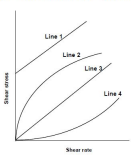
\includegraphics[width=0.5\linewidth]{figs/fig35.png}
     \caption{}
     \label{fig:placeholder}
 \end{figure}

\hfill [XE GATE 2017]

\begin{multicols}{2}
\begin{enumerate}
\item P-2, Q-4, R-3, S-1
\item P-1, Q-3, R-4, S-2
\item P-4, Q-2, R-1, S-3
\item P-4, Q-3, R-2, S-1
\end{enumerate}
\end{multicols}



    \item Water flowing at a rate of 1 kg/min is heated from 12 to 80 $^\circ$C with flue gas supplied at a rate of 3 kg/min. The temperature and specific heat of the flue gas are 180 $^\circ$C and 1.05 kJ/kg.K, respectively. If specific heat of water is 4.2 kJ/kg.K and the flow is parallel, then the logarithmic mean temperature difference will be $\underline{\hspace{2cm}}$ $^\circ$C. 
    \hfill[XE GATE 2017]

    \item The Lineweaver-Burk plot of an enzymatic reaction shows $V_{max}$ of 160 $\mu$mol/l.min and $K_s$ of 60 $\mu$mol/l. For a substrate concentration of 40 $\mu$mol/l, the velocity of the reaction is estimated to be $\underline{\hspace{2cm}}$ $\mu$mol/l.min.
    \hfill[XE GATE 2017]

    \item Bread is wrapped in 0.1 mm thick cellophane film having water vapour permeability of $1.82 \times 10^{-10}$ m$^3$ water (STP)/s.m$^2$.atm at 38 $^\circ$C. If the surface area of pack, vapour pressure of water inside and outside of the pack is 0.20 m$^2$, 10 mm Hg and 5 mm Hg, respectively, the loss of water vapour at 38 $^\circ$C in g/day is $\underline{\hspace{2cm}}$.
    \hfill[XE GATE 2017]

    \item Match the following methods / system (column I) with the appropriate operations (column II).

    \begin{multicols}{2}
        \textbf{Column I}
        \begin{enumerate}[label=\Alph*.]
            \item Parboiling
            \item Reaming
            \item Milling
            \item Break rolls
            \item Unbaked products
            \item Crushing rolls
        \end{enumerate}

        \columnbreak

        \textbf{Column II}
        \begin{enumerate}[label=\arabic*.]
            \item Sugarcane juice extraction
            \item Hydrothermal treatment
            \item Oven milling
            \item Wet milling
            \item Barley processing
            \item Pulse milling
        \end{enumerate}
    \end{multicols}

    \hfill[XE GATE 2017]

    \begin{multicols}{2}
        \begin{enumerate}[label=(\Alph*)]
            \item P4, Q2, R3, S6, T2, U1
            \item P4, Q5, R3, S1, T4, U1
            \item P2, Q5, R3, S1, T4, U1
            \item P2, Q5, R3, S2, T6, U1
        \end{enumerate}
    \end{multicols}

    \item A 12 mm thick fish fillet having 80\% moisture content (wet basis) is to be frozen using a plate freezer. The plates are maintained at -35 $^\circ$C. Assume the heat transfer coefficient, initial freezing temperature and latent heat of fusion are 2.0 W/m$^2 \cdot$K, -2 $^\circ$C and 330 kJ/kg, respectively. If the density and thermal conductivity of frozen fish fillet are 1050 kg/m$^3$ and 1.48 W/m$\cdot$K, respectively, the time required to freeze the fillet from the initial freezing temperature is $\underline{\hspace{2cm}}$ h.
    \hfill [XE GATE 2017]

    \item A suspension containing $2 \times 10^4$ spores of organism A having a $D_{121.1^\circ C}$ value of 1.5 min and $3 \times 10^5$ spores of organism B having a $D_{121.1^\circ C}$ value of 0.8 min is heated at a constant temperature of 121.1 $^\circ$C. The heating time needed to obtain a probability of spoilage `1 in 1000' is $\underline{\hspace{2cm}}$ min.
    \hfill [XE GATE 2017]

    \item In an evaporation process, a compressor picks up 0.05 m$^3$ air in each revolution and compresses 500 kg of air per minute. If the specific volume of air is 0.9 m$^3$/kg, then the compressor speed is $\underline{\hspace{2cm}}$ rpm.
    \hfill [XE GATE 2017]

    \item For a soybean oil extraction system, solvent : soy ratio is maintained at 0.5 : 1 (w/w). Original seed contains 18\% oil (w/w). If the meal (soy solid) after final desolventization contains 1\% residual oil (w/w, oil-free meal basis), then the effectiveness of the solvent (kg oil/kg solvent) in the extraction process is $\underline{\hspace{2cm}}$.
    \hfill [XE GATE 2017]

\item Rossby Number is the ratio of
\begin{multicols}{2}
\begin{enumerate}
    \item Coriolis Force to Inertial Force
    \item Inertial Force to Coriolis Force
    \item Gravitational Force to Coriolis Force
    \item Viscous Force to Inertial Force
\end{enumerate}
\end{multicols}

 \hfill [XE GATE 2017]


\item Kuroshio Current and Gulf Stream are
\begin{multicols}{2}
\begin{enumerate}
    \item EBC, WBC
    \item EBC, EBC
    \item WBC, WBC
    \item WBC, EBC
\end{enumerate}
\end{multicols}
[WBC: Western Boundary Current, EBC: Eastern Boundary Current]

 \hfill [XE GATE 2017]


\item The velocity of a tsunami wave in an ocean basin of depth 1 km is \quad ms$^{-1}$
[Density of seawater: 1025 kg m$^{-3}$. g: 10 ms$^{-2}$]

\hfill [XE GATE 2017]

\item A thin iceberg is observed to move southeastward in the Arctic Ocean. If the surface current is wind driven, the prevailing wind is
   
    
    \hfill [XE GATE 2017]
    
  
    \begin{multicols}{4}
        \begin{enumerate}
            \item Easterly
            \item Northerly
            \item Southerly
            \item Westerly
        \end{enumerate}
    \end{multicols}
    
    \item Equatorial Kelvin and Rossby waves respectively propagate
   
    
    \hfill [XE GATE 2017]
    
    
    \begin{multicols}{4}
        \begin{enumerate}
            \item Westward and Eastward
            \item Eastward and Westward
            \item Westward and Westward
            \item Eastward and Eastward
        \end{enumerate}
    \end{multicols}
    
    \item The largest contributor to the atmospheric greenhouse effect is
  
    
    \hfill [XE GATE 2017]
    
 
    \begin{multicols}{4}
        \begin{enumerate}
            \item CO$_2$
            \item N$_2$
            \item CH$_4$
            \item H$_2$O
        \end{enumerate}
    \end{multicols}
    
    \item If $T_v$, $T$, $T_w$ and $T_d$ denote virtual, dry bulb, wet bulb and dew point temperatures of a moist air parcel, then the correct order of their values is
   
    
    \hfill [XE GATE 2017]
    

    \begin{multicols}{2}
        \begin{enumerate}
            \item $T_v > T > T_w > T_d$
            \item $T_v \geq T \geq T_w \geq T_d$
            \item $T_v > T \geq T_w \geq T_d$
            \item $T > T_v > T_w > T_d$
        \end{enumerate}
    \end{multicols}
    
    \item Burning of fossil fuel is increasing the concentration of CO$_2$ in the atmosphere. A consequence of this is
    
    
    \hfill [XE GATE 2017]
    
    
\begin{multicols}{2}
        \begin{enumerate}
            \item Ocean water which is presently basic will drift towards pH neutral
            \item Ocean water which is presently acidic will become more acidic
            \item No effect on ocean pH
            \item Ocean water which is presently slightly basic will become more basic
        \end{enumerate}
    \end{multicols}
\item Mixed layer depths measured in the Pacific Ocean in two different years are schematically shown in the figure below.
Years P and Q belong to

 \hfill [XE GATE 2017]

\begin{figure}[H]
    \centering
    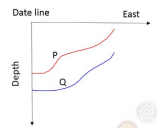
\includegraphics[width=0.5\linewidth]{figs/fig36.png}
    \caption{}
    \label{fig:placeholder}
\end{figure}
\begin{multicols}{2}
\begin{enumerate}
    \item P: El-Ni\~no, Q: La-Ni\~na
    \item P: La-Ni\~na, Q: El-Ni\~no
    \item P: El-Ni\~no, Q: QBO
    \item P: QBO, Q: La-Ni\~na
\end{enumerate}
\end{multicols}

 \item Average surface temperatures of the Sun and the Earth are 6300 K and 285 K, respectively. The ratio of the wavelength of peak radiation of the Earth to that of the Sun is $\underline{\hspace{2cm}}$.
 
    \hfill [XE GATE 2017]

    \item In the month of April, the mixed layer in the Arabian Sea received a net heat flux of 50 W m$^{-2}$. If the mixed layer depth is 50 m, the increase in temperature at the end of April is $\underline{\hspace{2cm}}$ $^\circ$C.  

    Density of seawater: 1025 kg m$^{-3}$, Density of freshwater: 1000 kg m$^{-3}$, Specific heat of seawater: 4200 J kg$^{-1}$ K$^{-1}$, Latent heat of evaporation: $2.45 \times 10^6$ J kg$^{-1}$.  
    
    \hfill [XE GATE 2017]

    \item The thickness of an atmospheric layer between 600 hPa and 500 hPa is 1.5 km. If the layer is isothermal, then its temperature is $\underline{\hspace{2cm}}$ K.  

    Gas constant of air: 287 J kg$^{-1}$ K$^{-1}$; g = 10 m s$^{-2}$.  
    
    \hfill [XE GATE 2017]

    \item At 17$^\circ$N, a mass of fluid is moving under geostrophic balance at 0.3 m s$^{-1}$ towards east. Suddenly the pressure gradient force becomes zero. Then the fluid will  

    \begin{enumerate}
        \item continue to move towards the east at 0.3 m s$^{-1}$  
        \item undergo circular motion with radius of about 17 km  
        \item undergo circular motion with radius of about 7 km  
        \item move towards south  
    \end{enumerate}

    (Angular velocity of the Earth: $7.27 \times 10^{-5}$ rad s$^{-1}$)  
    
    \hfill [XE GATE 2017]

    \item At 45$^\circ$N, wind is blowing northward and its magnitude decreases eastward from 10 m s$^{-1}$ to 1 m s$^{-1}$ over a distance of 1000 km. The relative vorticity of the flow is $\underline{\hspace{2cm}} \times 10^{-5}$ s$^{-1}$.  

    (Angular velocity of the Earth: $7.27 \times 10^{-5}$ rad s$^{-1}$)  
    
    \hfill [XE GATE 2017]

\item Sea surface height anomalies at the locations A, B, C and D are -10, -15, 5 and 0 cm respectively.
\begin{figure}[H]
    \centering
    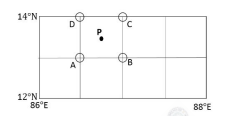
\includegraphics[width=0.5\linewidth]{figs/fig37.png}
    \caption{}
    \label{fig:placeholder}
\end{figure}
The magnitude of geostrophic velocity at P is \underline{\hspace{2cm}} m s$^{-1}$.
[Take 1$^\circ$ = 100 km, $g=10~m~s^{-2}$. Angular velocity of the Earth: $7.27 \times 10^{-5}~rad~s^{-1}$]

\item In a severe tropical cyclone, 250 mm of rainfall occurs in an area having a radius of 200 km. If the energy supplied to the system from this rainfall is $N$ times the energy of one atomic bomb ($=1.5\times10^{15}$ kJ), then the value of $N$ is \underline{\hspace{2cm}}.

[Density of freshwater: 1000 kg m$^{-3}$, Specific heat of seawater: 4200 J kg$^{-1}$ K$^{-1}$, Latent heat of evaporation: $2.45\times10^{6}$ J kg$^{-1}$]

\hfill [XE GATE 2017]


\item A student wants to numerically solve the linear 1-D advection equation $\dfrac{\partial q}{\partial t}+c\dfrac{\partial q}{\partial x}=0$, where $c=300$ m s$^{-1}$. The value of the maximum time-step the student can consider according to CFL criterion for a spatial resolution of 3 km is

\hfill [XE GATE 2017]

\begin{multicols}{2}
\begin{enumerate}
\item 15 s
\item 10 s
\item 25 s
\item 20 s
\end{enumerate}
\end{multicols}


\item Planets in the solar system are in radiative equilibrium. Let $S_0$, $\alpha$, $T_0$ and $R$ denote solar constant, albedo, average temperature and radius of a planet, respectively, and $\sigma$ is Stefan’s constant. Then the energy balance of this planet is given by the expression

\hfill [XE GATE 2017]

\begin{multicols}{2}
\begin{enumerate}
\item $(1-\alpha)S_0=4\,\sigma\,T_0^{4}$
\item $(1-\alpha)S_0=2\,\sigma\,T_0^{4}$
\item $\alpha S_0=\sigma\,T_0^{4}$
\item $\pi R^{2}(1-\alpha)S_0=4\,\sigma\,T_0^{4}$
\end{enumerate}
\end{multicols}


\item A cumulonimbus cloud forms by an air parcel rising from the sea level with an initial temperature and specific humidity of $27^\circ$C and 20 g kg$^{-1}$, respectively. Assume that moist static energy is conserved in this cloud. Then the cloud temperature at an altitude of 15 km is \underline{\hspace{2cm}} K.

[Specific heat of dry air at constant pressure: 1005 J kg$^{-1}$ K$^{-1}$, Specific heat of water vapour at constant pressure: 1850 J kg$^{-1}$ K$^{-1}$; $g=10$ m s$^{-2}$, Latent heat of evaporation: $2.45\times10^{6}$ J kg$^{-1}$]

\hfill [XE GATE 2017]

\item If $u_g$ and $v_g$ are respectively zonal and meridional components of a flow field in geostrophic balance, then the divergence of this flow is  

\hfill [GATE XE 2017] 

\begin{multicols}{2}
\begin{enumerate}
\item $0$  
\item $\dfrac{u_g}{\rho} \dfrac{\partial r}{\partial x}$  
\item $-\dfrac{1}{\rho f} \dfrac{\partial^2 p}{\partial y^2}$  
\item $-\dfrac{v_g}{\rho f} \dfrac{\partial r}{\partial y}$  
\end{enumerate}
\end{multicols}

{\small [ $x,y,f,u,v,p,\rho$ are zonal distance, meridional distance, Coriolis parameter, pressure and density, respectively ]}  

 

\item During the Indian summer monsoon season, depressions do not intensify to tropical cyclones because  

P: Indian sub-continent is very hot and large land-sea temperature difference pulls depressions quickly to land before they can intensify into cyclones.  
Q: SST cooling due to strong monsoonal winds prevents cyclone formation.  
R: SST cooling due to strong monsoonal winds prevents cyclone formation.  
S: Strong zonal wind shear during the monsoon season does not allow warm core formation.  

Which of the above statement(s) is/are correct?  

\hfill [GATE XE 2017]  


\begin{multicols}{2}
\begin{enumerate}
\item P \& Q  
\item Only R  
\item Only S  
\item R \& S  
\end{enumerate}
\end{multicols}


\item Which among the following statement(s) is (are) correct.  

P: ENSO and El-Nino are the same and refer to the warming of Equatorial Eastern Pacific SST.  
Q: ENSO is an atmosphere-ocean coupled phenomenon and El-Nino is its oceanic part.  
R: ENSO is an atmospheric phenomenon and El-Nino is an ocean phenomenon.  
S: ENSO is the oscillatory component of El-Nino having a period of 4-7 years.  

\hfill [GATE XE 2017]  

\begin{multicols}{2}
\begin{enumerate}
\item P \& R  
\item Only Q  
\item P, Q and S  
\item R \& S  
\end{enumerate}
\end{multicols}



\end{enumerate}

\end{document}
